% Re-defined by TIAN ZICHEN
\documentclass[12pt]{report}

%% Useful packages
\usepackage[a4paper,top=3cm,bottom=3cm,left=3.5cm,right=3cm,marginparwidth=1.75cm,headheight=22pt]{geometry}
\usepackage{amsmath}
\usepackage{cite}
\usepackage{courier}
\usepackage[export]{adjustbox}
\usepackage[labelfont=bf, textfont=bf]{caption}
\usepackage{graphicx}
\usepackage{hyperref}
\usepackage{float}
\usepackage{setspace}
\usepackage{subfigure}
\usepackage{setspace}
\usepackage{lipsum}
\usepackage{fancyhdr} % Fancy header
\usepackage{url}
\usepackage{tabularx}
\usepackage[utf8]{inputenc}
\usepackage{mathptmx} %Times Font

%==== Header and Footer configure ====
% Turn on the style
% Clear the header and footer
\fancypagestyle{plain}{
\fancyhf{} % Clear header footer
\fancyhead[R]{\bf \textsl{\leftmark} \vspace{0.1in}}
\fancyfoot[R]{\thepage}
% Set the right side of the footer to be the page number
\renewcommand{\headrulewidth}{2pt}
}
% For those Chapter* (Can't use \leftmark to call their chapter name directly)
\fancypagestyle{addin}{
\fancyhf{} % Clear header footer
\fancyhead[R]{\bf \textsl{\leftmark} \vspace{0.1in}}
% Set the right side of the footer to be the page number
\fancyfoot[R]{\thepage}
\renewcommand{\headrulewidth}{2pt}
}



%==== Overall Config ====
\setlength{\parindent}{0in}
% \setlength{\fboxsep}{-0.3in}%
\setlength{\fboxrule}{0.5pt}%
\pagestyle{plain}


\begin{document}
%==== FRONT PART====
\begin{titlepage}

\begin{figure}[h!]
\centering

\includegraphics[width=0.8\textwidth]{Title/NTU_logo.png}
\caption*{}
\label{fig:entropy} 
\end{figure}

\vspace{1in}

\centering
\Huge{\textbf{Lane-Aware Image Enhancement\\for Lane Detection in Rain}}\\[2in]

\LARGE{\textbf{TIAN ZICHEN}}\\[2in]

\normalsize{\textbf{SCHOOL OF ELECTRICAL AND ELECTRONIC ENGINEERING}}\\[0.2in]

% \textbf{A DISSERTATION SUBMITTED IN PARTIAL FULFILMENT OF\\
% THE REQUIREMENTS FOR THE DEGREE OF\\
% MASTER OF SCIENCE IN DIGITAL MEDIA TECHNOLOGY}\\[0.25in]

\large{\textbf{2021}}
\end{titlepage}
\newpage

%\begingroup
%\let\cleardoublepage\clearpage

\pagenumbering{roman}

\renewcommand*\contentsname{\centering Table of Contents}
\tableofcontents
\newpage

%=== FRONT PART ===
%=== ABSTRCT ===
\newpage
\fancypagestyle{addin}{
\fancyhead[R]{\bf \textsl{ABSTRACT} \vspace{0.1in}}
}
\chapter*{\centering Abstract}
\addcontentsline{toc}{chapter}{Abstract}
% \vspace{-0.3in}
\begin{spacing}{1.5}
\setlength{\parskip}{0.3in}
\thispagestyle{addin}

In recent years, auto-driving is becoming a hot topic. Auto-driving cars utilize in-vehicle cameras to capture the surrounding environment images and use algorithms to extract useful information from images. One of the most critical issues to be solved in auto-driving is lane detection and road marking recognition. By implementing lane and road marking detection algorithms, surrounding traffic symbols can be recognized and used to help the human driver avoid accidents. 

Two central problems are in such process: 1) the curved road is not easy to detect; 2) the extreme weather condition may distort the image captured by cameras, thus hard to recognize.

In this paper, a network structure RVPGNet, based on previous work VPGNet, is described to address above mentioned problems. It employs multi-task to do lane detection and road marking classification tasks simultaneously and utilizes the vanishing point to guide the lane prediction. To save computational resources, we use an innovative 4-tiling layer. We use a new feeding scheme to utilize the vanishing point better and avoid training being trapped at the saddle point. The network is implemented and experimented with the CAFFE framework and is transplanted to the PyTorch framework. In the CAFFE implementation, a $97.19\%$ accuracy is achieved in multi-label classification. In the test of extreme weather conditions, the network achieves as high as $93.35\%$ to $99.73\%$ $F_1$ score in the rainy and low-brightness situation.

% The PyTorch implementation still needs improvements. It is available on GitHub now waiting for further researchers and contributors.

% \par
% \thispagestyle{addin} % NOTICE: to make another page show!
% \textbf{Keywords:} Dissertation, keywords.
\end{spacing}
\newpage
%=== END OF ABSTRACT ===

%=== FRONT PART ===
%=== ACKNOWLEDGEMENT ===
\fancypagestyle{addin}{
\fancyhead[R]{\textsl{ACKNOWLEDGEMENT} \vspace{0.1in}}
}
%\begin{center}
\chapter*{Acknowledgement}
\thispagestyle{addin}
%\end{center}
\addcontentsline{toc}{chapter}{Acknowledgement}

Here.
\newpage
%=== END OF ACKNOWLEDGEMENT  ===

%=== FRONT PART ===
%=== ACRONYMS ===
\fancypagestyle{addin}{
\fancyhead[R]{\bf \textsl{ACRONYMS} \vspace{0.1in}}
}
%\begin{center}
\chapter*{\centering Acronyms}
\begin{spacing}{1.5}
\setlength{\parskip}{0.3in}
\thispagestyle{addin}
%\end{center}
\addcontentsline{toc}{chapter}{Acronyms}

% Please add the following required packages to your document preamble:
% \usepackage{graphicx}
\begin{table}[ht]
\centering
% \resizebox{\textwidth}{!}{%
\begin{tabular}{ll}
\textbf{VP} & Vanishing Point \\
\textbf{VPGNet} & Vanishing Point Guided Neural Network \\
\textbf{RVPGNet} & Refined Vanishing Point Guided Neural Network \\
\textbf{NN} & Neural Network \\
\textbf{ML \& DL} & Machine Learning and Deep Learning \\
\textbf{ADAS} & Advanced Driver Assistance System \\
\textbf{FCN} & Fully Convolutional Network \\
\textbf{CNN} & Convolutional Neural Network \\
\textbf{RCNN} & Region Based Convolutional Neural Network
\end{tabular}%
% }
\end{table}

\end{spacing}
\newpage
%=== END OF ACRONYMS ===

%=== FRONT PART ===
%=== SYMBOLS ===
\fancypagestyle{addin}{
\fancyhead[R]{\textsl{SYMBOLS} \vspace{0.1in}}
}
%\begin{center}
\chapter*{Symbols}
\thispagestyle{addin}
%\end{center}
\addcontentsline{toc}{chapter}{Symbols}

Symbols goes here.
\newpage
%=== END OF ACKNOWLEDGEMENT  ===



\renewcommand{\listfigurename}{\centering List of Figures}
\listoffigures
\addcontentsline{toc}{chapter}{Lists of Figures}
\newpage

\renewcommand{\listtablename}{\centering List of Tables}
\listoftables 
\addcontentsline{toc}{chapter}{Lists of Tables}
\newpage

%\endgroup

%==== MAIN PART ====

\pagenumbering{arabic}
%=== CHAPTER ONE (1) ===
%=== INTRODUCTION ===

\chapter{Introduction}
\begin{spacing}{1.5}
\setlength{\parskip}{0.3in}

The first chapter of the dissertation is almost invariably the Introduction. Generally, its purpose is to lead the readers into the problem you intend to attack in the project, to set the scene. The main points here consist of the background to the problem and your motivation in solving it. This then leads into the objectives and the scope of the project. It is good to conclude your Introduction with a section on the layout of the dissertation. It prepares the readers for what is to come.

\section{Background}

The era of the smart cars is coming, and Advanced-driver-assistance system plays an important role in it. Object detection technologies are used to improve the performance of Advanced-driver-assistance system.

Smart cars equipped with Advanced-driver-assistance system are popular now. With the development of smart driving and Eco-energy technology, more and more companies began to produce and sale the newly designed, electric-driven, smart-driving assistant cars. Leading companies like TESLA, NIO and QuantumScape made hundreds of thousands of cars every year (till 2020)~\cite{petranek2015we}. With these cars bought by more and more families, the smart cars are no longer a concept for common people, but becomes a daily necessities for everyone, as an alternative to a traditional car. Compared with traditional mechanical fuel vehicle, new smart vehicles have many advantages. They are 'new', not only because they are driven by electric energy, but also because they are equipped with intelligent driving assistance systems, which is usually called Advanced-driver-assistance system (ADAS).

\begin{figure}[ht]
\centering
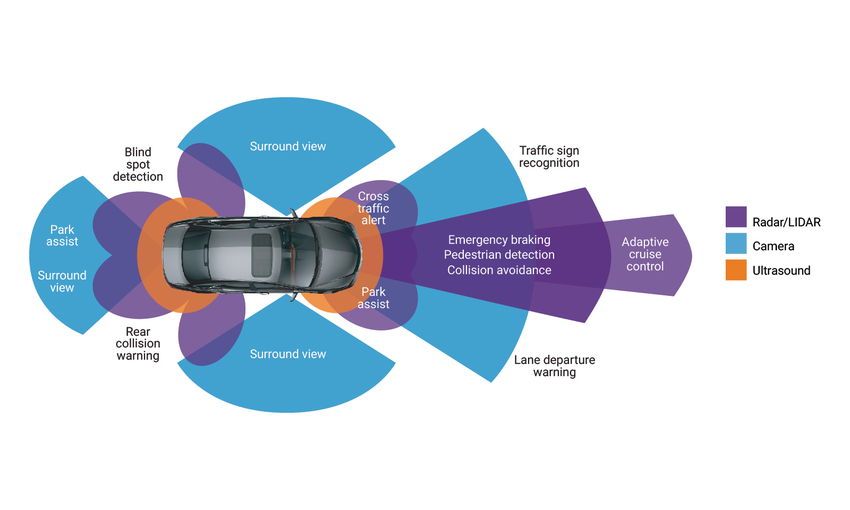
\includegraphics[width=5.5in, fbox]{Chapter1/adas.jpg}
\caption{Advanced-driver-assistance system (ADAS)~\cite{adas}}
\label{fig:adas} 
\end{figure}

ADAS system can reduce road fatalities by minimizing human error. Basic architecture of ADAS system can be shown in \autoref{fig:adas}. Firstly, it utilizes the sensors (LIDAR, in-vehicle camera, GPS) to collect the surrounding obstacle or global position information. Secondly, by combining the information grabbed from all the sensors, the ADAS system can get information that is useful for driving, such as driver's state, current geographical position of cars, the road congestion, potential obstacles on the road, and the trending of road~\cite{morignot2014arbitration}. Such information can be further utilized by the driver or the analysis system to avoid potential dangerous. Because the safety problem is one of the most severe unsolved problems of the traditional human controlled vehicles, ADAS can significantly reduce the death rate related to fatal driving~\cite{brookhuis2001behavioural}.

To improve the performance of ADAS system is an object detection task. ADAS systems use in-vehicle cameras to capture the real-time images of roads~\cite{ziebinski2016survey}. Captured images will be handled by detection module, which recognizes lane outlines and road markings, and then respond to drivers accordingly. This is basically a object detection problem in computer vision area. 

Our work is to solve the problems raised from aforementioned situation, and can be used to improve the performance of ADAS system. 

\section{Motivation}

There are several common issues in aforementioned detection process. 

First is extreme weather and bad illumination conditions. In raining days, images captured by ADAS’s camera may be blurry or be stained by raindrops, and the water on the road may lead to reflection of lights, as shown in figure TBC. In dusk, sun is dim, and the scene is dark-some. The road markings and lane outlines cannot be distinguished from background easily, as shown in figure TBC. With such distortions, the detection algorithm cannot see roads accurately. Consequently, taking measures to denoising is of vital importance. 

Second is curved road. Traditional lane detection algorithms usually work well on straight lane but will meet performance drop once the road turns quickly. One sample of such roads is as in TBC. VPGNet~\cite{lee2017vpgnet} used vanishing point information to solve this problem. Vanishing point is the visual intersection of two parallel lines~\cite{barnard1983interpreting}, here it is treated as the unseen end of the road.  Inspired by the intuition that human eyes utilize the vanishing point to predict the road trending, VPGNet tried to feed this information into neural network by multi-task method. They use multi-task because features employed by VP task, like road curving angle and trending, may also be useful in the detection of lanes and road markings. Based on this, we can expect that with VP information given, the Neural Network can converge better on the other two tasks (lane detection, road marking detection). But VPGNet’s VP feeding scheme is simple, not as efficient as expected. We proposed a new scheme to train with VP information.


Here is a sample of table in \autoref{tabelsample}

\begin{table}[ht]
\centering
\caption{A table without vertical lines.}
\label{tabelsample}
\begin{tabular}[t]{lcc}
\hline
&Treatment A&Treatment B\\
\hline
John Smith&1&2\\
Jane Doe&--&3\\
Mary Johnson&4&5\\
\hline
\end{tabular}
\end{table}%

\section{Motivation}



\section{Objectives and Specifications}



\section{Major contribution of the Dissertation}



\section{Organisation of the Dissertation}


\end{spacing}
%=== END OF CHAPTER ONE ===
\newpage



%=== CHAPTER TWO (2) ===
%=== Literature Review ===

\chapter{Literature Review}
\label{cha:literature}
\begin{spacing}{1.5}
\setlength{\parskip}{0.3in}

\section{Introduction}

Then comes the main part of your work. To lay the ground, there should first be a chapter on what has been done before on the problem - a Literature Review. This is an important section because it shows that you do not narrowly focus only on what you do, but are aware of the
related work elsewhere, some of which might be instructive to your solving the problem. It can also explain why you are taking the direction you do.

\section{An Overview}
\label{sec:LR_overview}

In the past few years, the lane detection method have been developed from classical ones to novel deep-learning based ones. In this section, I will give a brief review of the classical lane detection methods proposed, and also give a brief overview of the developments in the field of object detection.

\subsection{Classical Lane Detection}

There are several ways to get the information for lane detection and prediction usage, such as Monocular vision, stereo, LIDAR, inertial measurement unit (IMU) combined with information obtained from global positioning system (GPS) and high resolution digital maps. \cite{hillel2014recent}. In this work I focus on Monocular vision (Single camera).

In previous work, researchers found relation between wheeling and gaze direction when driving. Human employs the distant region to estimate the road curvature \cite{land1995parts}. Also, the gaze direction relies on the 'tangent point' on the inside of each curve when driving on curvature of the road ahead \cite{land1994we}. This gives possible to utilize the unseen vanishing point in lane prediction.

\subsection{Deep-learning based Lane Detection}

Lane and road marking detection tasks are within the scope of object detection, so algorithms popular in object detection have been implemented in lane detection \cite{tang2020review}. 

Recent years, with the DCNN like AlexNet \cite{krizhevsky2012imagenet} being brought up, deep learning has been driving significant progress in the object detection area. Later RCNN and its variants \cite{girshick2014rich, girshick2015fast, ren2015faster} integrates CNN with the region proposal selective search; GoogLeNet \cite{szegedy2015going} and VGGNet \cite{simonyan2014very} gained improvement with deeper encoder. With the network going deeper, computational efficiency becomes the main problem. More powerful network architectures such as ResNets \cite{he2016deep}, DenseNets \cite{huang2017densely} and Inception \cite{ioffe2015batch} have been proposed, which combine path blocks to reduce the number of parameters while improving the accuracy. Most recently, DETR \cite{carion2020end} combined the CNN with transformer architecture, taking the object detection problem as a set-set mapping and achieved promising results on big-object detection.

Lanes are thin and small objects, thus general methods sometimes work bad \cite{tang2020review}. There are some researches featured in picking out small items. U-Net \cite{ronneberger2015unet} extracts the feature map from encoding path and attach it with the decoding path, by which method the network can keep context for local features.

Efforts to use the neural network in lane detection tasks have also been proved solid. Work \cite{borji2016vanishing} first used the CNN structure to predict the vanishing point, and VPGNet \cite{lee2017vpgnet} employed vanishing point information by multi-task method to enhance the prediction of the lanes.

\section{Neural Network Basis}

Neural Network is the most distinguish deep learning architecture based on Neural units recent years. Compared with conventional machine learning and human-designed mathematical classification algorithms, deep learning on the Neural Network have many advantages. In this section, I will give the theoretical basis of the Neural Networks, and also explain how it works by introducing the back propagation mechanism.

\subsection{Machine Learning}

Compared with specific mathematical equations designed for different kinds of problems, the conventional machine learning are based on \textit{experience}. \textit{Experience} here means that: the machine learning computational models can learn the features from a given data set (learn the \textit{experience} from input), and do prediction or classification based on the that \textit{experience} for any inputs, whether have seen or unseen before.~\cite{mohri2018foundations}.

The process of learning the features can be seen as a clustering operation. Each input data can be mapped into a $n$-dimension vector, and each vector can be viewed as a point in the $n$-dimension hyperspace. \autoref{fig:2dcluster} and \autoref{fig:3dcluster} shows the $2D$ and $3D$ clustering process. Clustering is to group data points into different clusters in the hyperspace, and draw the hyperplane between such clusters. This hyperplane is the interface between classes. For example, in figure \autoref{fig:2dcluster}, 2 groups of data were divided by a linear line, and in figure \autoref{fig:3dcluster}, 2 groups of data were divided by a non-linear curved surface.

\begin{figure}[ht]
\centering
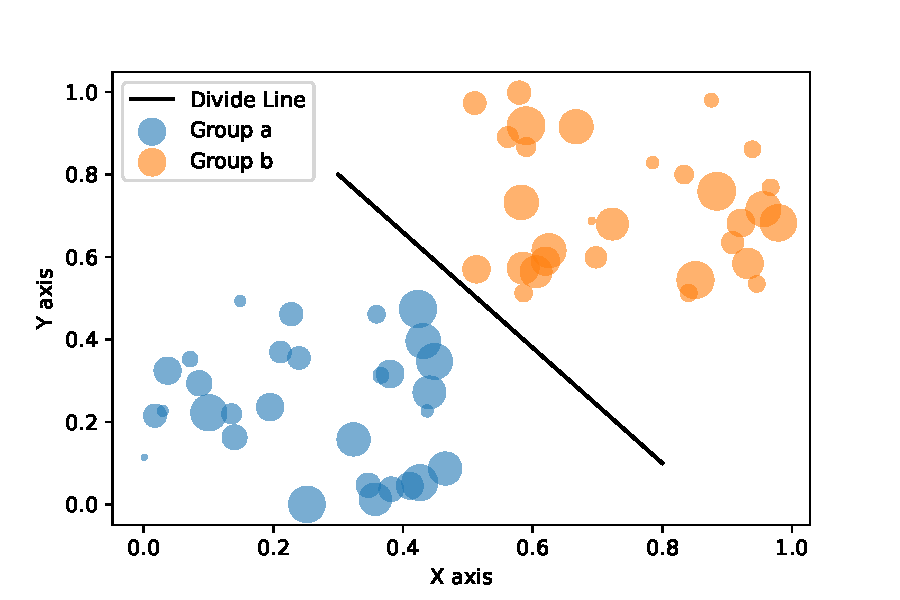
\includegraphics[width=0.99\textwidth, fbox]{Chapter2/2dcluster.pdf}
\caption{$2D$ Clustering}
\label{fig:2dcluster} 
\end{figure}

% \begin{figure}[ht]
% \centering
% \fbox{
% \includesvg[width=0.97\textwidth]{Chapter2/3dcluster.svg}
% }
% \caption{$2D$ Clustering}
% % \label{fig:2dcluster} 
% \end{figure}

\begin{figure}[ht]
\centering
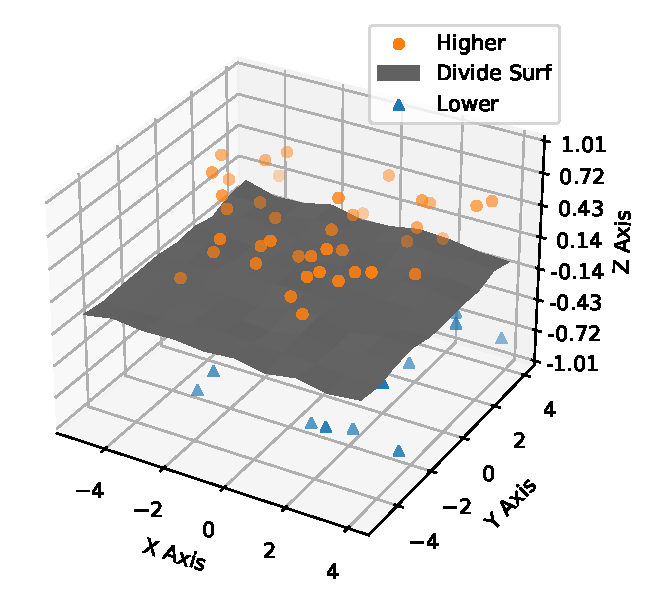
\includegraphics[width=0.6\textwidth, fbox]{Chapter2/3dcluster.pdf}
\caption{$3D$ Clustering}
\label{fig:3dcluster} 
\end{figure}

Above mentioned examples only calculate linear or non-linear division between two classes, but normally in real world applications, what needed are not limited to binary classification but usually multi-classification. In the machine learning, there are two solutions on multi-classification problem: 

1) \textit{Uncombined algorithms} will treat the multi-classification as a whole and finish training in only one phase, such as $N$-class SVM, decision trees. 

2) \textit{Aggregated algorithms} will split $N$ class classification into many binary classification, thus need multiple training phase. There are two types of aggregated algorithms: a) \textit{One-versus-one} calculate boundaries for every pair of classes, thus for $N$ class, it needs $N!=N*(N-1)*...*2*1$ calculations, as shown in \autoref{fig:121}. b) \textit{One-versus-others} calculate the boundary between the target class and all other data, thus for $N$ class, it needs to calculate $N$ boundaries, as shown in \autoref{fig:12all}. 

\begin{figure}[th]
    \centering
    \begin{subfigure}[b]{0.49\textwidth}
        \centering
        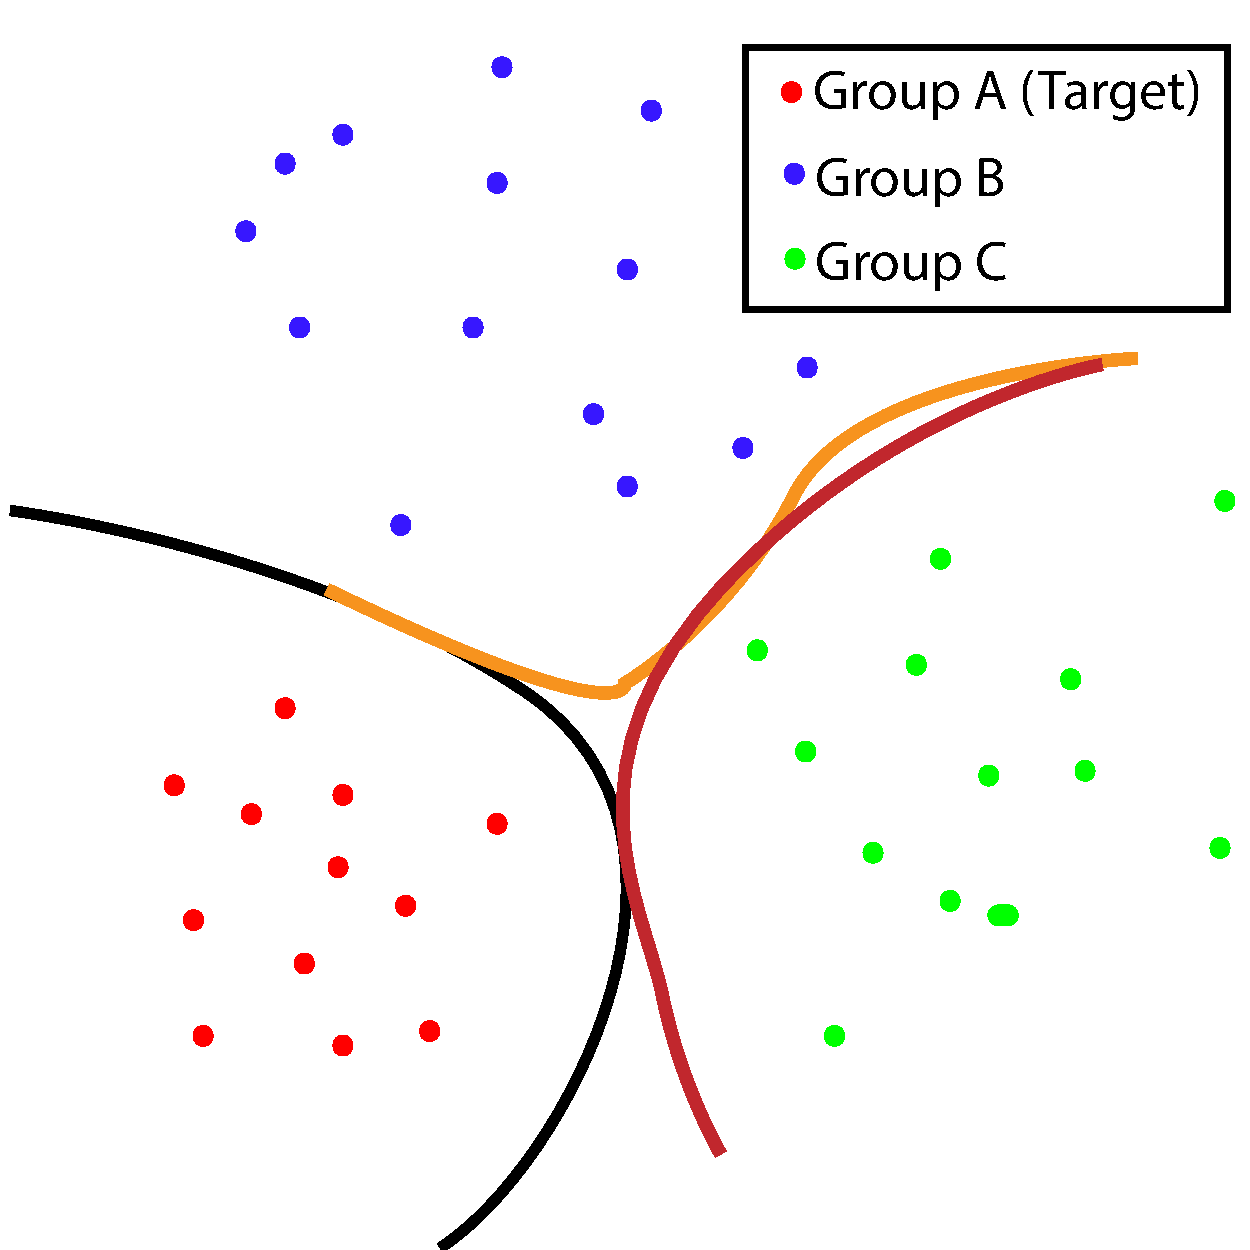
\includegraphics[width=2.7in, fbox]{Chapter2/1to1.pdf}
        \caption{One-to-one Multi-classification}
        \label{fig:121} 
    \end{subfigure}%
    ~
    \begin{subfigure}[b]{0.49\textwidth}
        \centering
        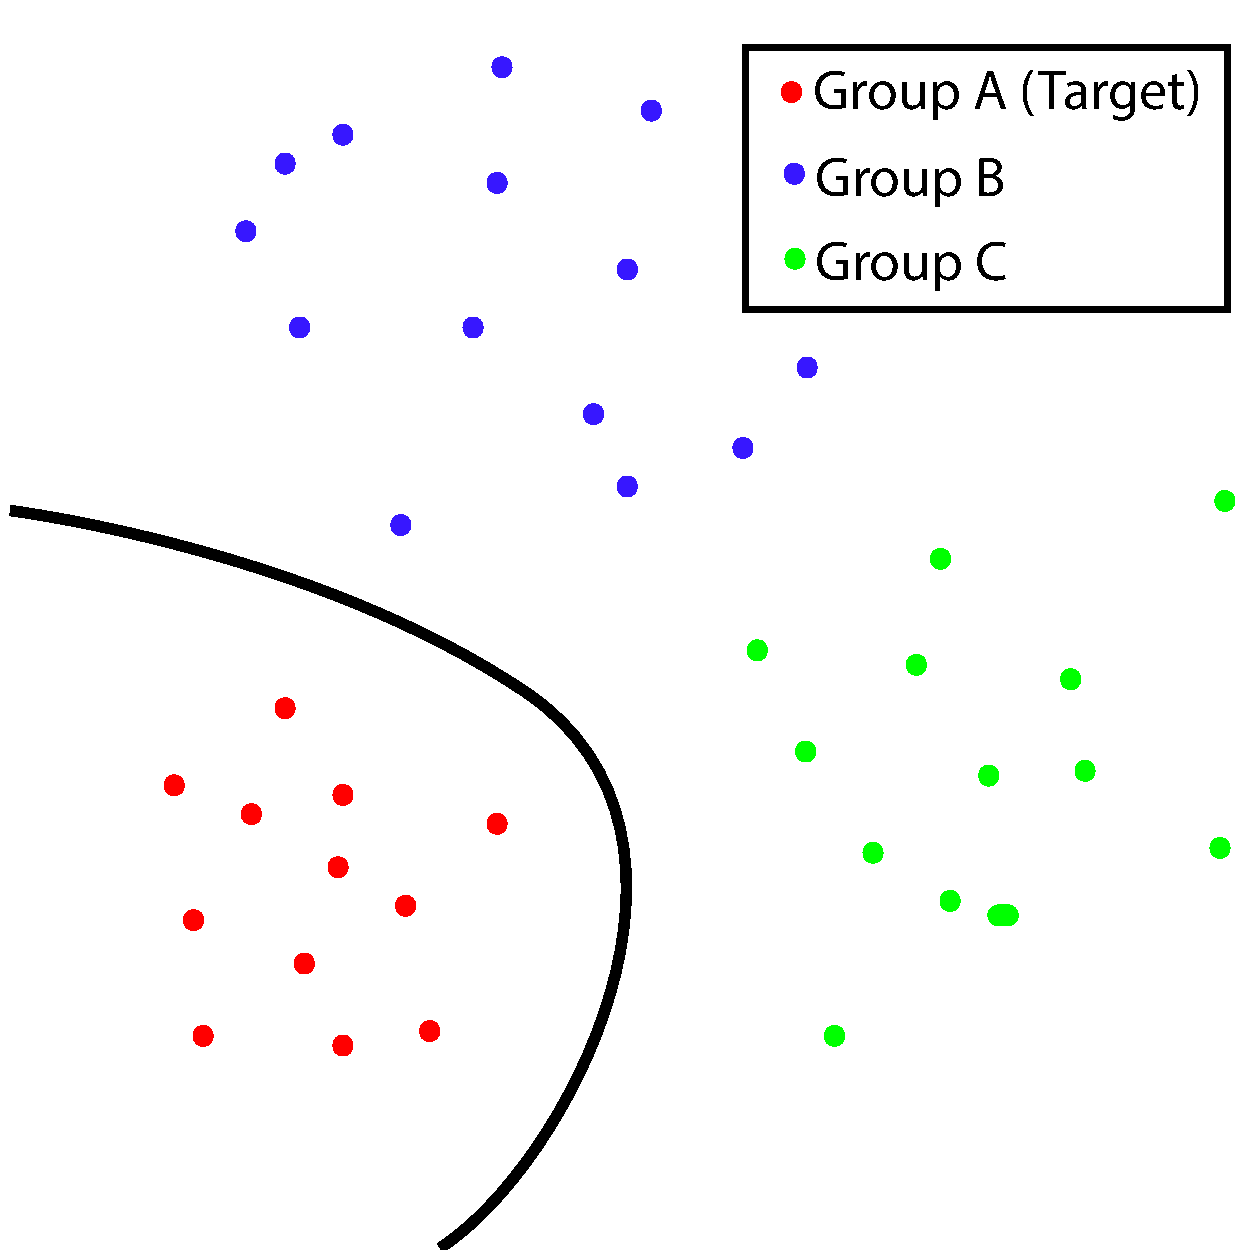
\includegraphics[width=2.7in, fbox]{Chapter2/1toall.pdf}
        \caption{One-to-all Multi-classification}
        \label{fig:12all} 
    \end{subfigure}
    \caption{Two Aggregated Algorithms}
\end{figure}


\subsection{Representation Learning and Deep Learning}

The main drawback of conventional machine-learning techniques is that they can not extract the features automatically and precisely from the raw input data. When using machine learning, engineers and researchers have to transform the raw data into normalized vectors that is suitable for training~\cite{ongsulee2017artificial}. Form the normalized vectors, the machine learning model can classify and do detection on the classify patterns.

Representation learning allows the machine to discover the best representation form of the raw data for machine learning training. Representation learning features that the algorithm can find and fit the best representation from the raw input data, no matter what format the input data is. Such representation of raw data is suitable for the further feature extraction~\cite{bengio2013representation}. For example, if the input is a gray-scale image, the output matrix after first representation layer would represent the position of edges and corners.

\begin{figure}[th]
    \centering
    \begin{subfigure}[b]{0.99\textwidth}
        \centering
        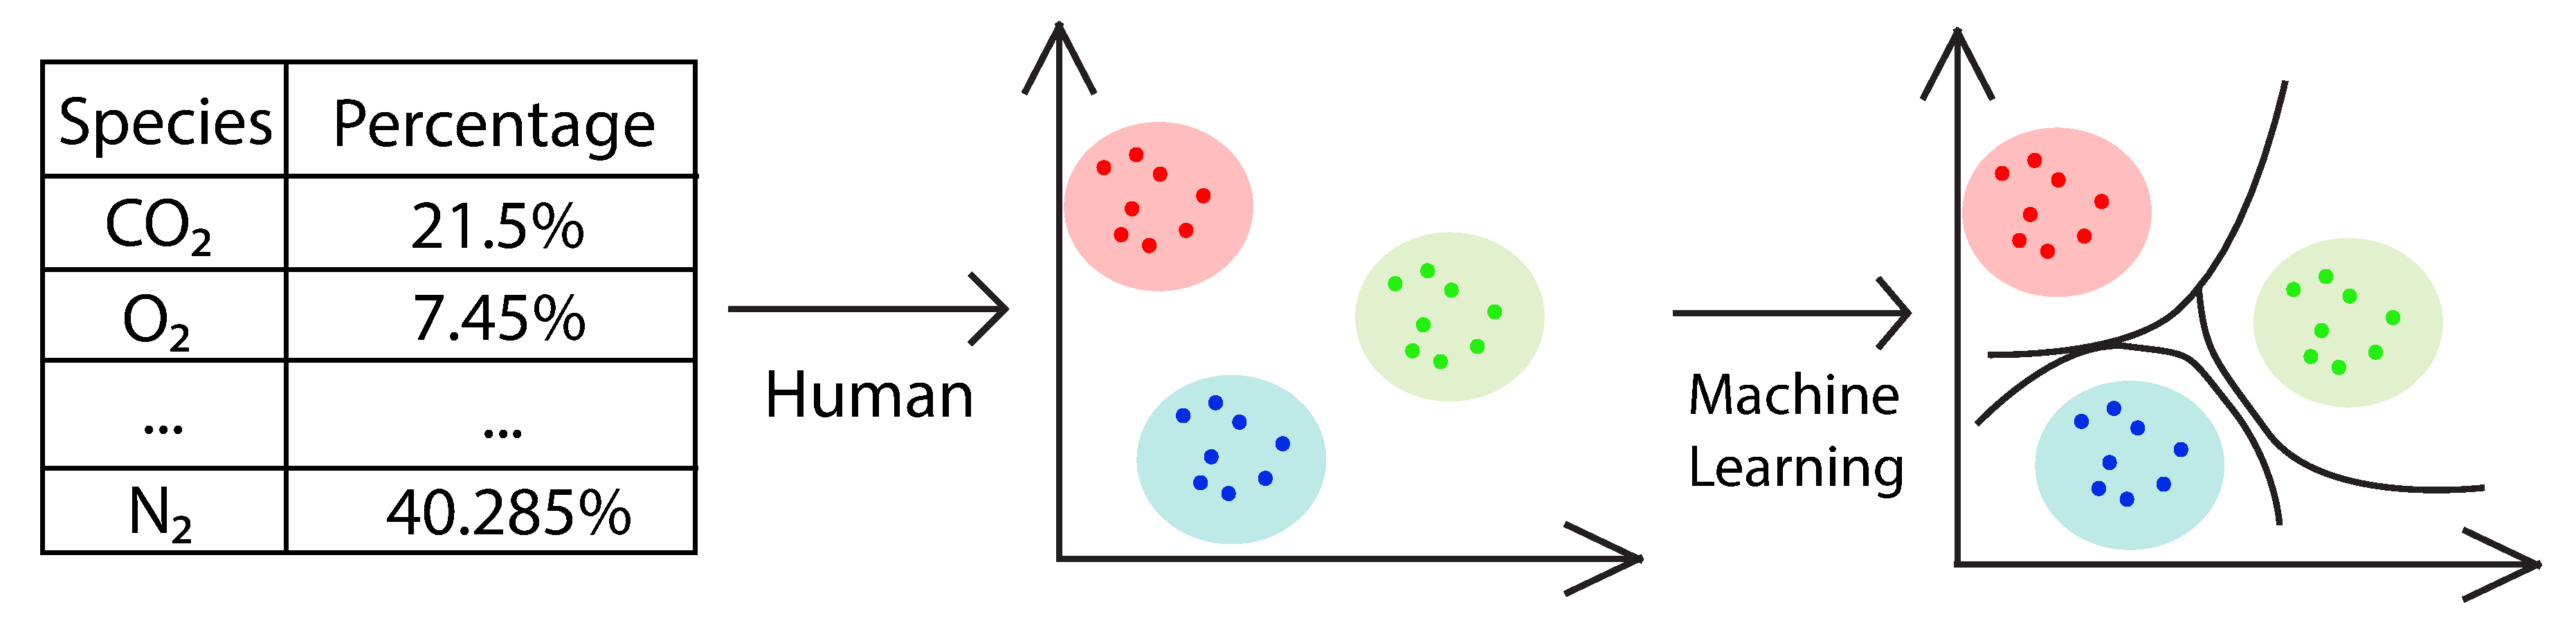
\includegraphics[width=0.98\textwidth, fbox]{Chapter2/Machine-Learing.pdf}
        \caption{Machine Learning: Human Data Centering}
        \label{fig:mldiagram} 
    \end{subfigure}%
    \\
    \begin{subfigure}[b]{0.99\textwidth}
        \centering
        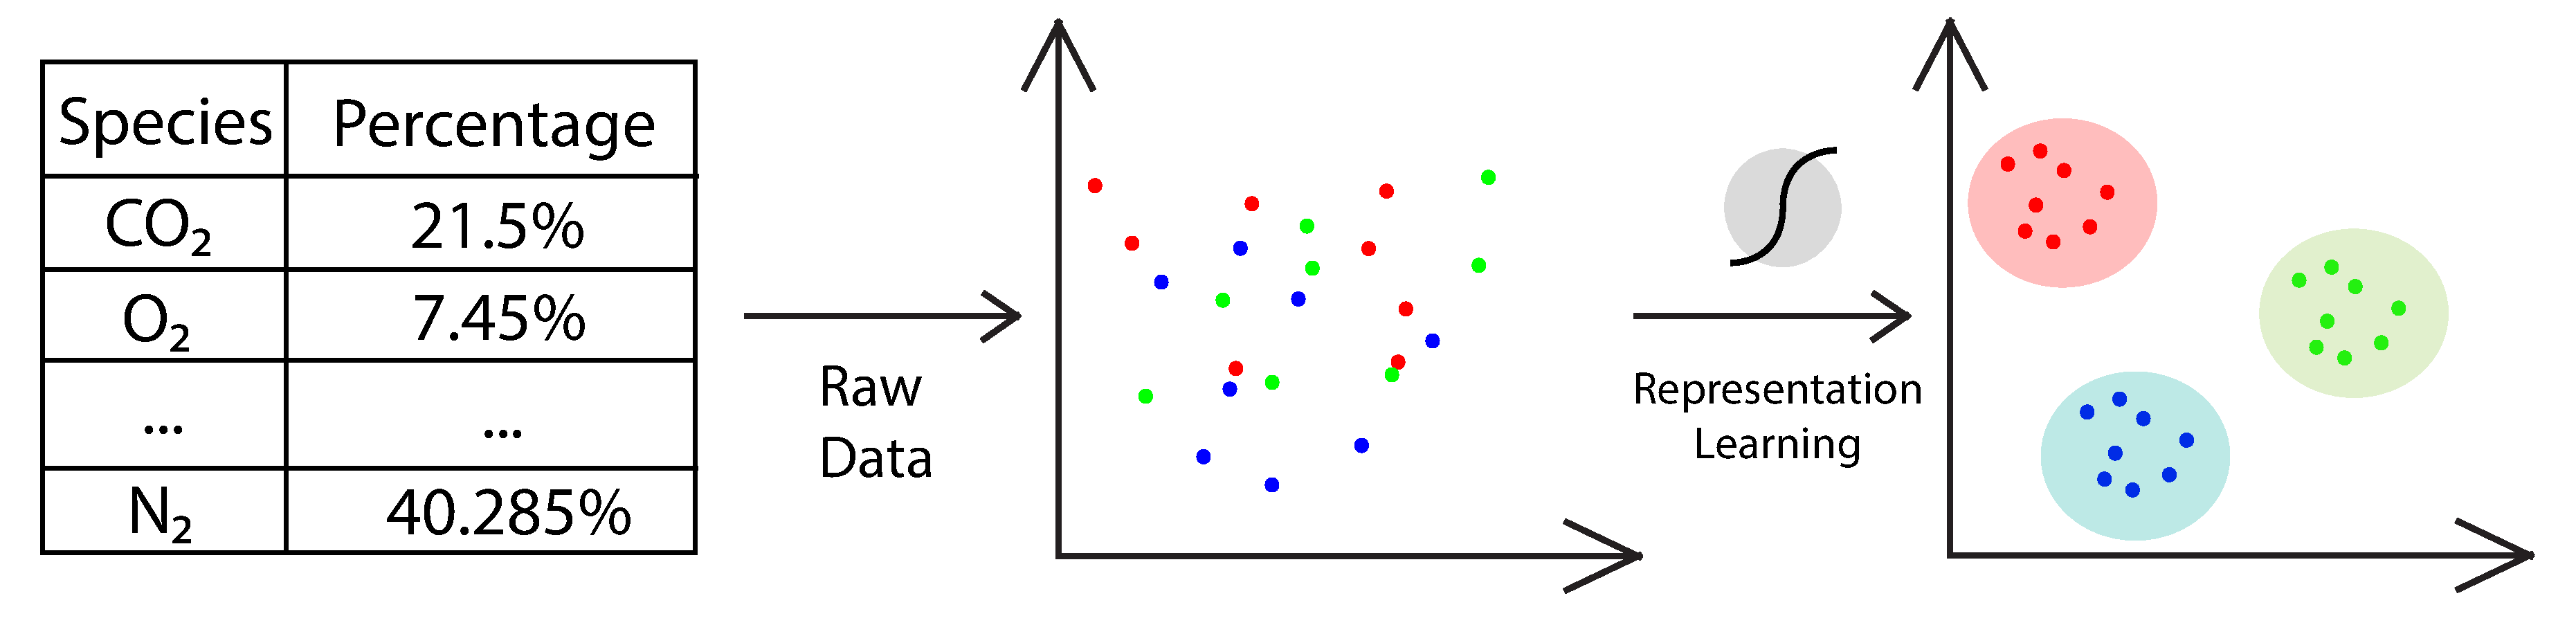
\includegraphics[width=0.98\textwidth, fbox]{Chapter2/Represent-Learing.pdf}
        \caption{Representation Learning: Auto Extraction}
        \label{fig:representdiagram} 
    \end{subfigure}
    \\
    \begin{subfigure}[b]{0.99\textwidth}
        \centering
        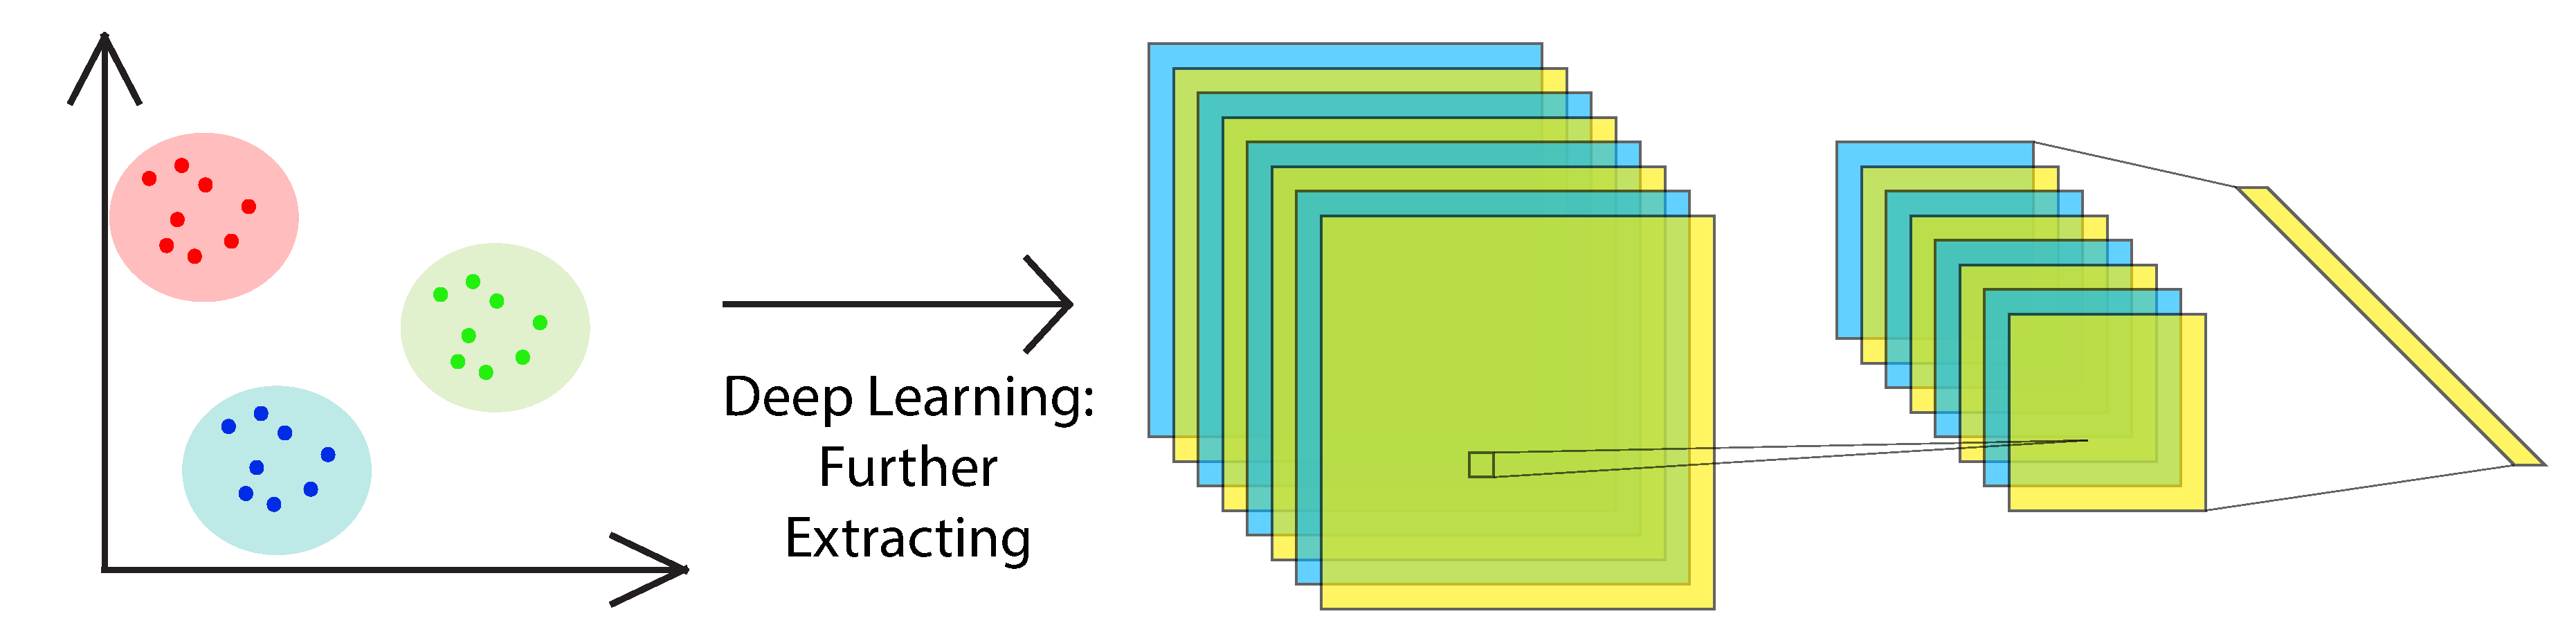
\includegraphics[width=0.98\textwidth, fbox]{Chapter2/Deep-Learing.pdf}
        \caption{Deep Learning: Further Extraction of Features}
        \label{fig:dldiagram} 
    \end{subfigure}%
    \caption{Comparison between Three Learning}
\end{figure}

Based on representation learning, the concept of deep learning was originally proposed in a study on Artificial Neural Network (ANNs) \cite{hinton2006reducing}. Basically, deep learning is a multi-layer and deeper version of representation learning. Deep learning can not only extract the features vectors from the first layer but also can go deeper, get more abstract high-level features. For example, if the input is a gray-scale image, the first layer of deep learning is just like the representation learning, extracting the position of edges and corners. The second layer of deep learning would extract the relative positions between the edges and corners, and the third layer of deep learning would treat edges and corners in similar shape as a group. With the network go deeper, such high-level abstract features can be sensed. In 2006, with a deep learning architecture called deep belief network (DBN) \cite{hinton2006fast} being invented by Hinton, the machine learning community rekindled heated discussion over deep-learning.

Give an example to illustrate the difference between the machine learning, representation learning and deep learning. For a chemical substances classification task, the input is the percentage of each components in a chemical mixture. When using machine learning algorithms like SVM, researchers have to re-form and normalize the input data, into a sparse data space, and should do multi-phase training for multi-classification (\autoref{fig:mldiagram}). When using representation learning methods, the input data can be raw data that has not been pre-processed (\autoref{fig:representdiagram}), such raw data will be mapped to high-dimension space by non-linear neural units. When using deep learning, the extracting layer goes deeper, thus can get more abstract features (\autoref{fig:dldiagram}).

Deep learning~\cite{lecun2015deep} is composed by simple non-linear \textit{Neural Unit} in each level. \textit{Neural Unit} is described in \autoref{subsec:neural_unit}. Deep learning uses the back propagation and feedforward mechanism to optimize the non-linear parameters of \textit{Neural Unit} from front to end. Propagation and feedforwad are described in \autoref{subsec:back_propagation}.


\subsection{Supervised, Unsupervised and Reinforcement Learning}

Machine learning algorithms can be classified into three main categories, according to the training data form and the learning mechanism of the algorithm: the supervised learning, the unsupervised learning and the reinforcement learning \cite{mohri2018foundations}. Between supervised learning and unsupervised learning, there are also semi-supervised learning.

Supervised learning is trained on labeled input and output~\cite{sen2020supervised, kotsiantis2007supervised}. Each input data $D_i$ is paired with a label or ground-truth value $L_i$, thus the training data should be in the format: $(D_i, L_i), i \in \mathbb{Z}$. The supervised learning aims to predict the corresponding label $l_i$ for each new input $d_i$. Supervised learning can be divided into two types: 

\begin{enumerate}
    \item Regression, when the label set $\{L_i\} = \mathbb{R}$, in which $\mathbb{R}$ is continuous real number set.
    \item Classification, when the label set $\{L_i\} = \mathbb{A}$, in which $\mathbb{A}$ is a set of discrete values $\{\alpha_1, \alpha_2, ...\}$ representing different classes.
\end{enumerate}

Unsupervised learning is to cluster unlabeled data set into different groups according to their feature\cite{meena2019survey}. It analyzes the bounding of a given vector set $\{D_1, D_2, ...,D_n\}$ (the training data), divide the set into $n$ groups $\{G_1, G_2, ..., G_n\}$, and tell if a new unseen data $d_i$ belongs to or not belongs to certain class $G_i$.

\begin{figure}[ht]
\centering
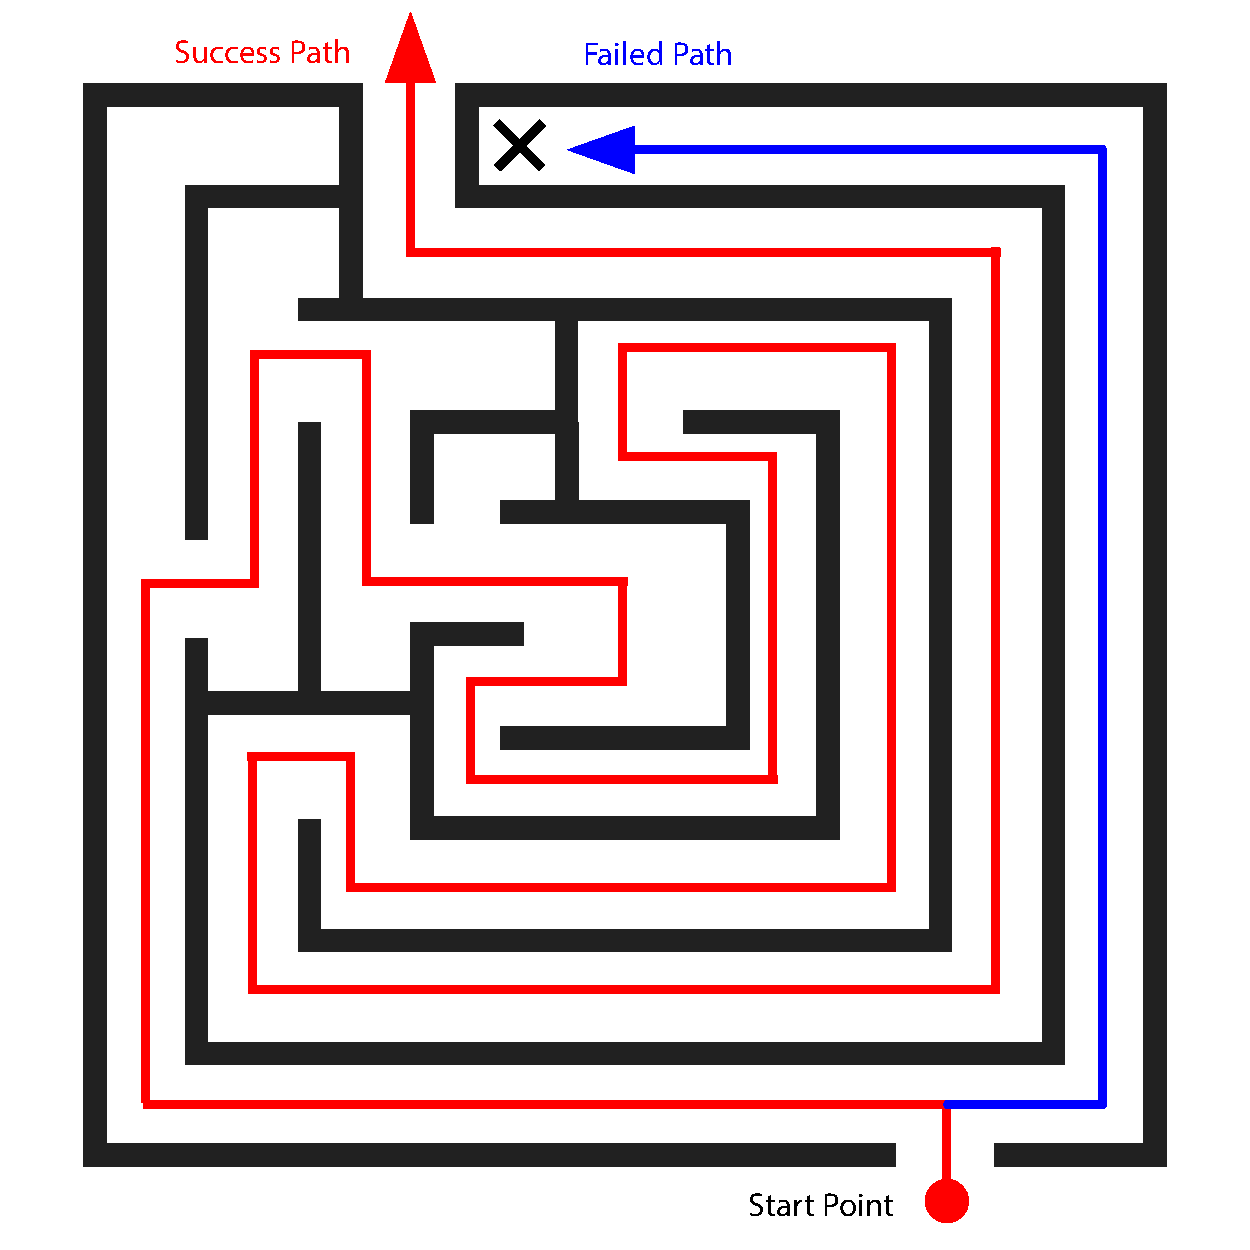
\includegraphics[width=0.75\textwidth, fbox]{Chapter2/reinforcement.pdf}
\caption{Reinforcement Learning: Maze Game Decisions}
\label{fig:reinforcement} 
\end{figure}

Reinforcement learning is to make the agent to play a game, or to perform a series of actions to reach to a certain goal~\cite{barto2004reinforcement}. The model will face a game-like situation, and make a consequence of decision to achieve the highest game score, as shown in~\autoref{fig:reinforcement}. First, the agent will observe the environment $\{\vec{E_i}\}$, which is a set of vectors representing the surrounding conditions. Second, the agent will conduct some action $\vec{a_i}$, and receive the reward/punishment score $\tau_i$. The aim of reinforcement learning is to find set of actions $\{\vec{a_i}\}, i \in (1,N)$, and such actions should satisfy the condition as described in~\autoref{eq:reinforce}.

\begin{equation}
\label{eq:reinforce}
   z = \argmax_{\{\vec{a_i}\}} \sum_{i=1}^{N} \tau_i
\end{equation}

Semi-supervised learning is to train the model on partially labelled data set~\cite{zhu2009introduction, zhu2005semi}. This method is a intermediate product of supervised learning and unsupervised learning. It addresses the problem that the fully labelled training data is hard to get, usually taking a lot of time to annotating all the data manually. If given a small set of labelled data set $\mathbb{D}_{label} = \{(D,L)\}$ along with a large set of unlabeled data set $\mathbb{D}_{unlabel} = \{D\}$, the semi-supervised learning can utilize the $\mathbb{D}_{label}$ to get the center of clusters, and utilize the $\mathbb{D}_{unlabel}$ to make the problem into a clustering problem.

\subsection{Neural Unit}
\label{subsec:neural_unit}

\begin{figure}[ht]
\centering
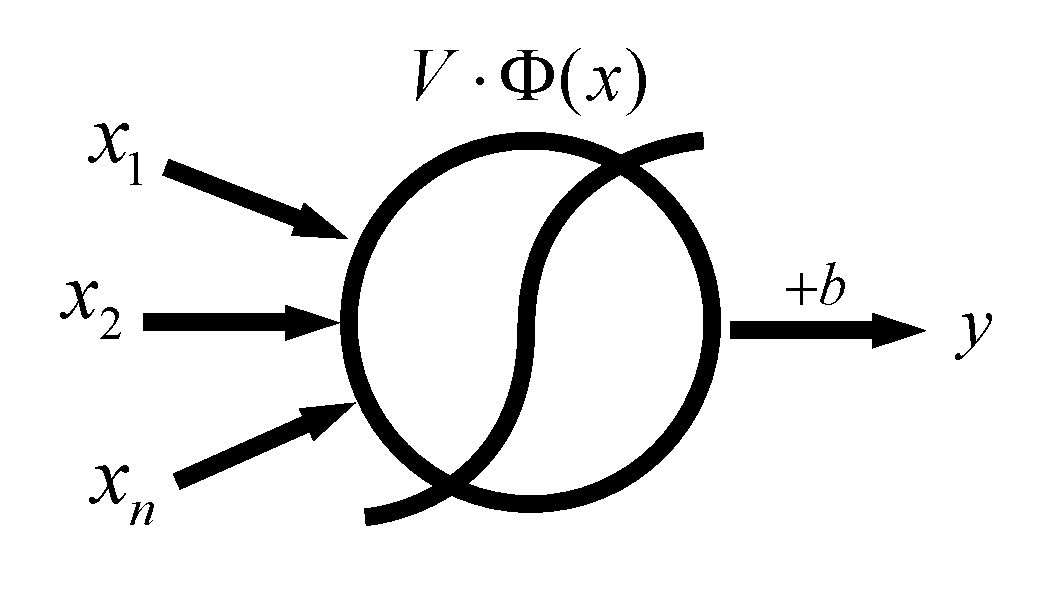
\includegraphics[width=0.5\textwidth, fbox]{Chapter2/neuralunit.pdf}
\caption{Neural Unit}
\label{fig:neuralunit} 
\end{figure}

The most basic unit that constructs the neural network is rather simple that is only a non-linear function with $n$ inputs and 1 output~\cite{bengio2017deep}, as shown in~\autoref{fig:neuralunit}. 

The function of input and output is as~\autoref{eq:neuralunit} shown. 

\begin{equation}
\label{eq:neuralunit}
    f(x)=b+V \cdot \Phi (c+W \vec{x})
\end{equation}

The $\Phi (\cdot)$ is the activation function, which could be some non-linear functions like \textit{Sigmoid} (\autoref{eq:sigmoid}), \textit{ReLU} (\autoref{eq:relu}) or \textit{Tanh} (\autoref{eq:tanh}). The image for the activation functions are shown in~\autoref{fig:activationfunc}. The activation function maps the input to another data space which is easier to perform classification. 



\begin{gather}
% \vspace{-0.3in}
   \Phi_{Sigmoid}(x)=\frac{1}{1+e^{-x}} \label{eq:sigmoid}\\
   \Phi_{ReLu}(x)=max(0,x) \label{eq:relu}\\
   \Phi_{Tanh}(x)=\frac{e^{x}-e^{-x}}{e^{x}+e^{-x}} \label{eq:tanh}
\end{gather}

\begin{figure}[th]
    \centering
    \begin{subfigure}[b]{0.49\textwidth}
        \centering
        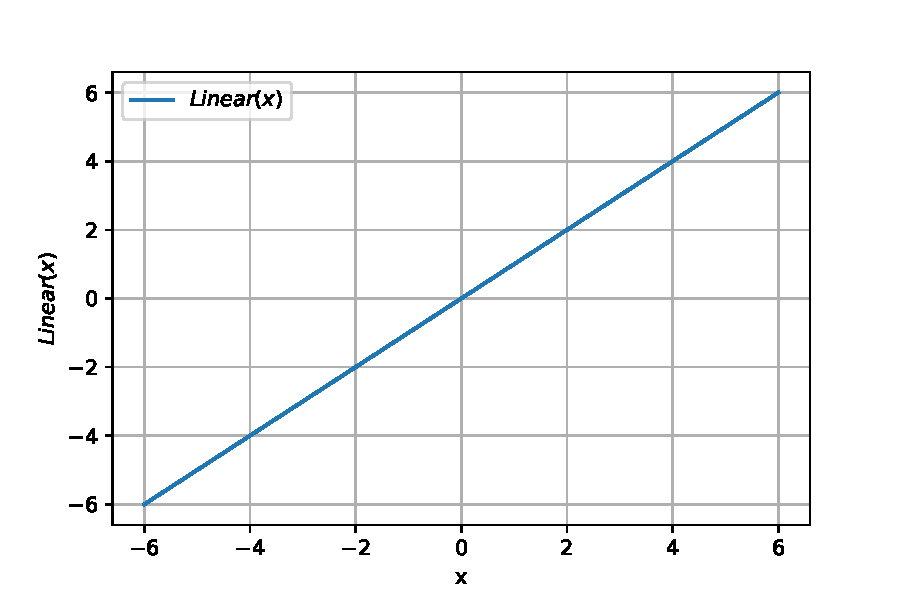
\includegraphics[width=2.7in, fbox]{Chapter2/linear.pdf}
        \caption{Linear}
    \end{subfigure}%
    ~
    \begin{subfigure}[b]{0.49\textwidth}
        \centering
        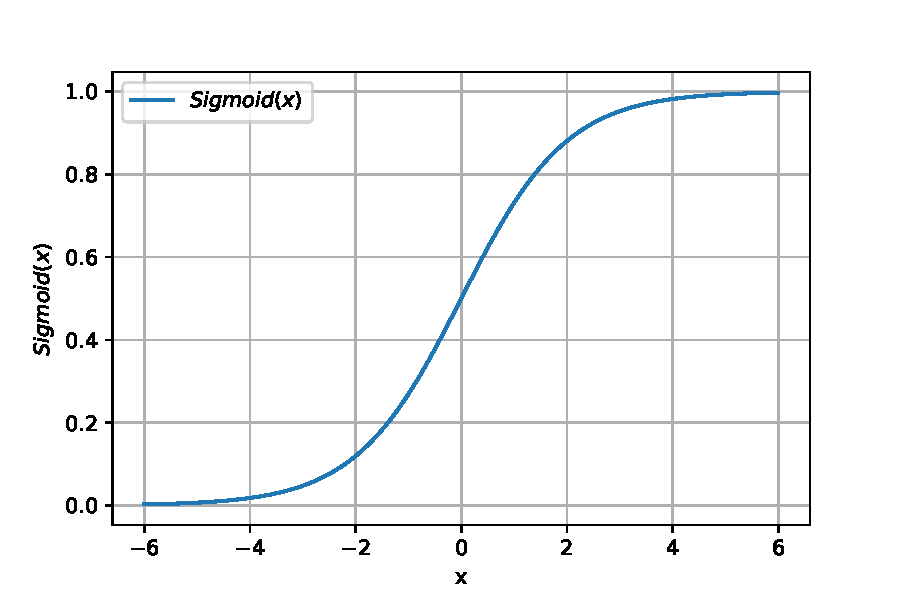
\includegraphics[width=2.7in, fbox]{Chapter2/sigmoid.pdf}
        \caption{Sigmoid}
        % \label{fig:sigfunc} 
    \end{subfigure}
    \\
    \begin{subfigure}[b]{0.49\textwidth}
        \centering
        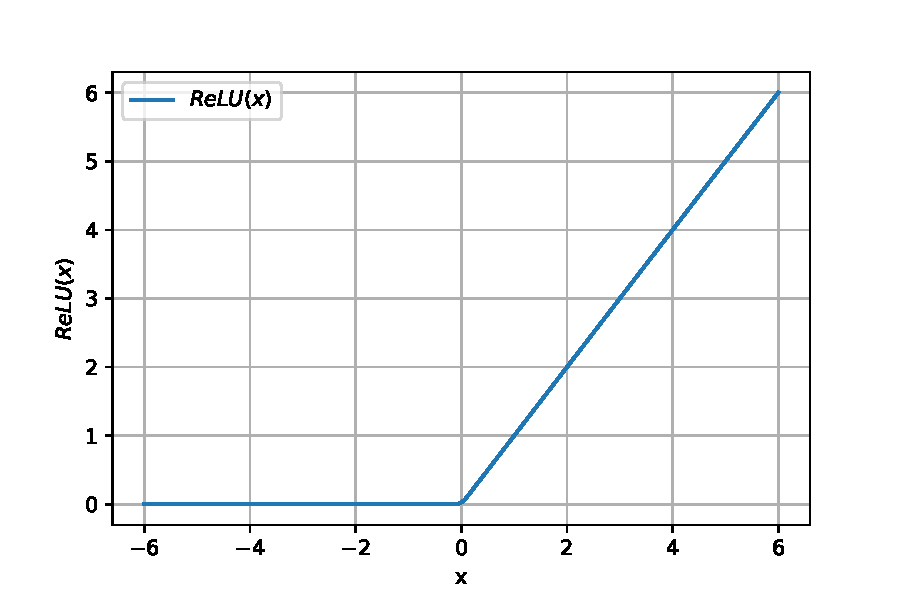
\includegraphics[width=2.7in, fbox]{Chapter2/ReLu.pdf}
        \caption{Rectified Linear Unit (ReLU)}
        % \label{fig:relufunc} 
    \end{subfigure}%
    ~
    \begin{subfigure}[b]{0.49\textwidth}
        \centering
        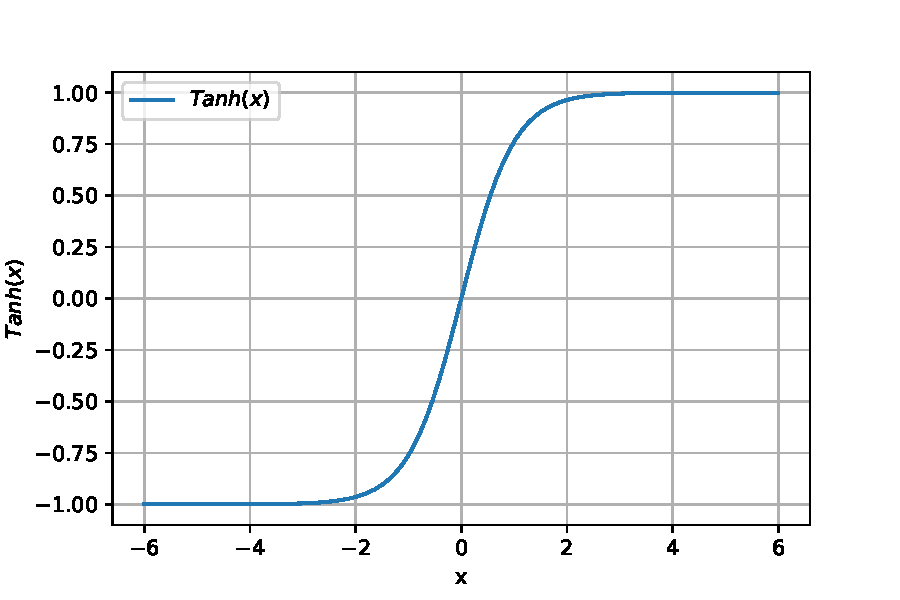
\includegraphics[width=2.7in, fbox]{Chapter2/tanh.pdf}
        \caption{Hyperbolic Tangent (Tanh)}
        \label{fig:tanhfunc} 
    \end{subfigure}
    \caption{Four Common Activation Functions}
    \label{fig:activationfunc} 
\end{figure}

For example, as shown in~\autoref{fig:activationlayer}, the blue line and red line in the input layer represents the input data. The division line is a curve between the two classes. After the activation layer (\textit{Sigmoid} function), the 2-D input space is transformed into a 3-D shape so that the examples from two classes can be separated linearly (the black line in center image in~\autoref{fig:activationlayer} is the division line). The image is edited based on the Christopher Olah's origin version in  \href{http://colah.github.io/posts/2014-03-NN-Manifolds-Topology/}{http://colah.github.io}. The author has posted many insightful images, and these images are broadly used by Y.Lecun and Yoshua.B in their publications~\cite{bengio2017deep, lecun2015deep}. The $W_i$ is the weight of the $i$-th neural unit, which is the main parameter adjusted by back propagation process.


\begin{figure}[th]
\centering
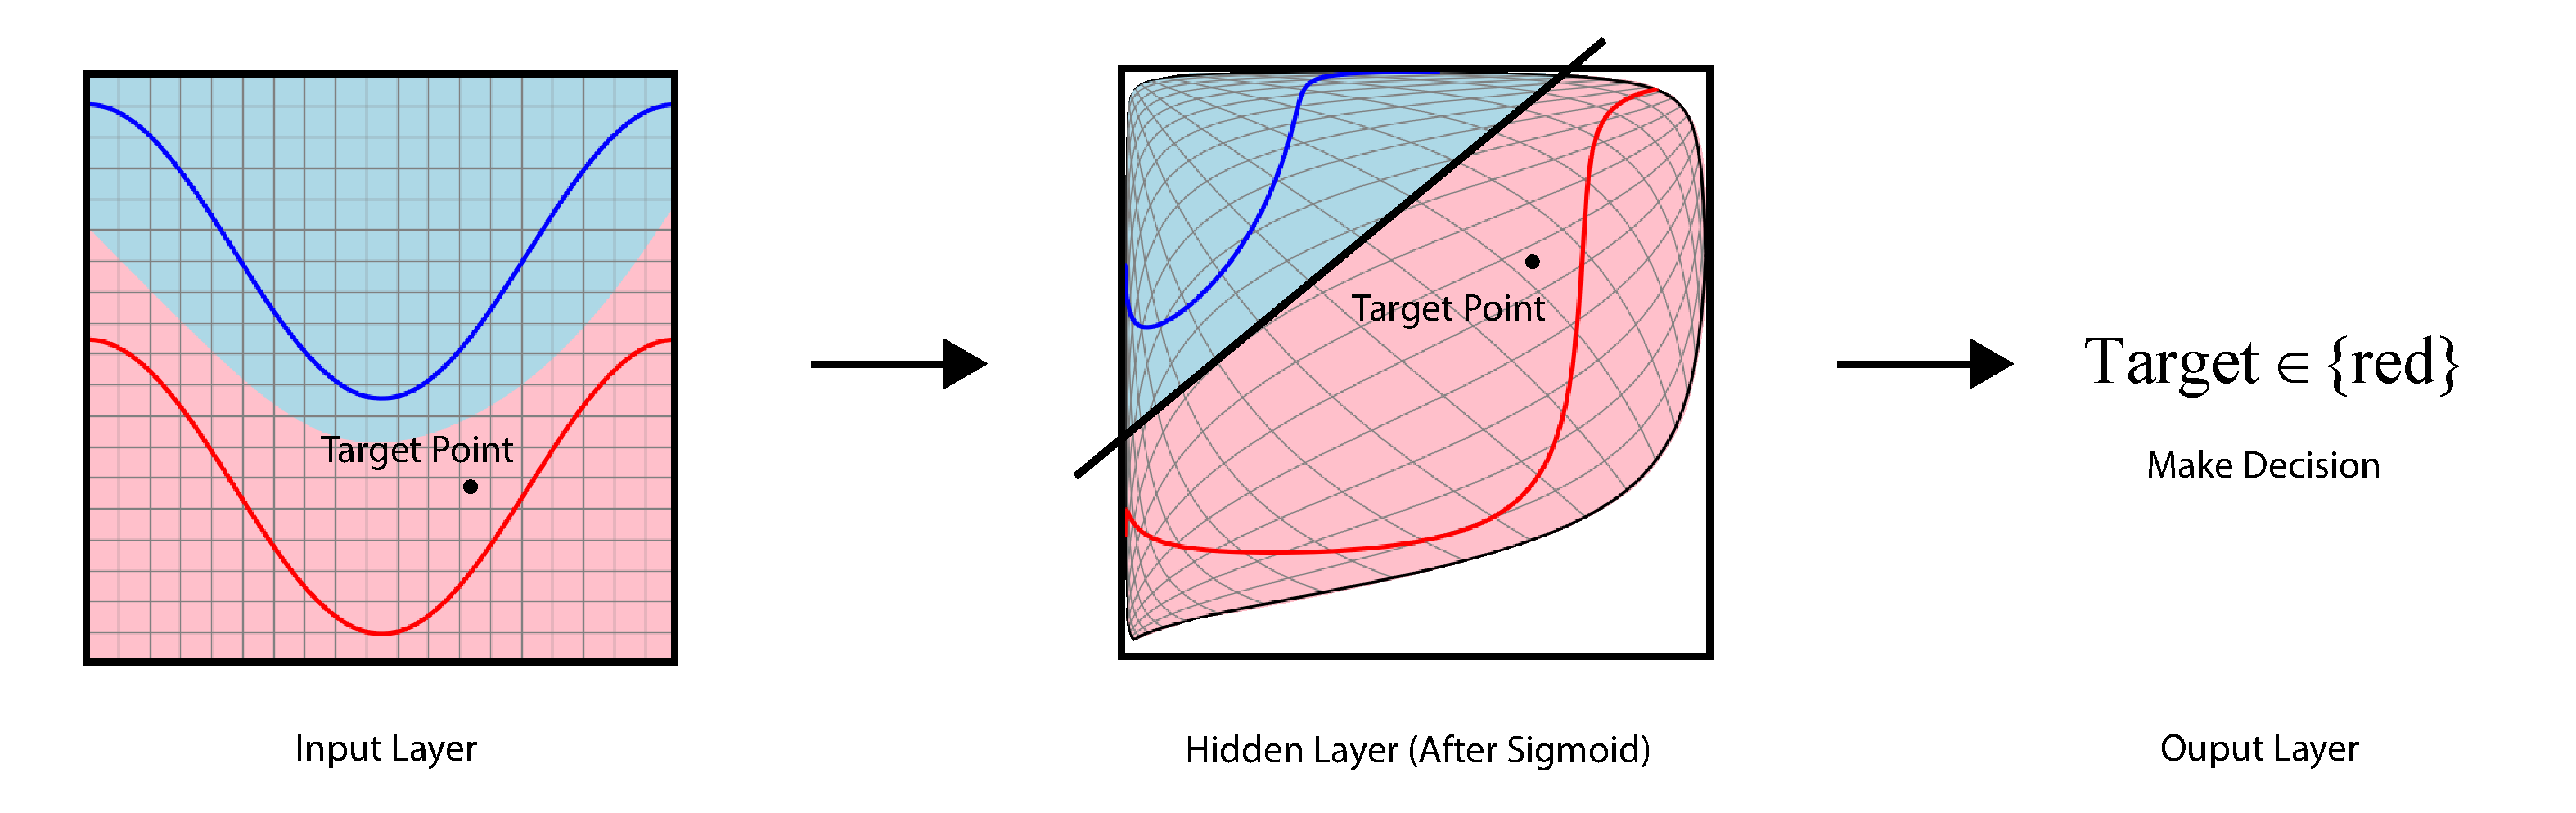
\includegraphics[width=0.99\textwidth, fbox]{Chapter2/activation.pdf}
\caption{Activation Kernal: Map to Nonlinear Data for Linear Decision~\cite{olah2014neural}}
\label{fig:activationlayer} 
\end{figure}

Any single layer in deep learning are made up by the non-linear neural units. As shown in~\autoref{fig:simplenn}, the input layer consists two neural units; the hidden layer (defined as those nodes not input either output), and it consists 9 nodes; the output layer consists only one node. Usually the output layer may consist of many nodes, in which case the \textit{flatten layer}, \textit{softmax layer} or other logistic regression functions are needed at the end of neural network, to make the output match with real-world case. And the parameter $W_i$, the weight of nodes, is the main part adjusted in the training process. This process is called feed-forward back propagation, which will be discussed in~\autoref{subsec:back_propagation}

\begin{figure}[th]
\centering
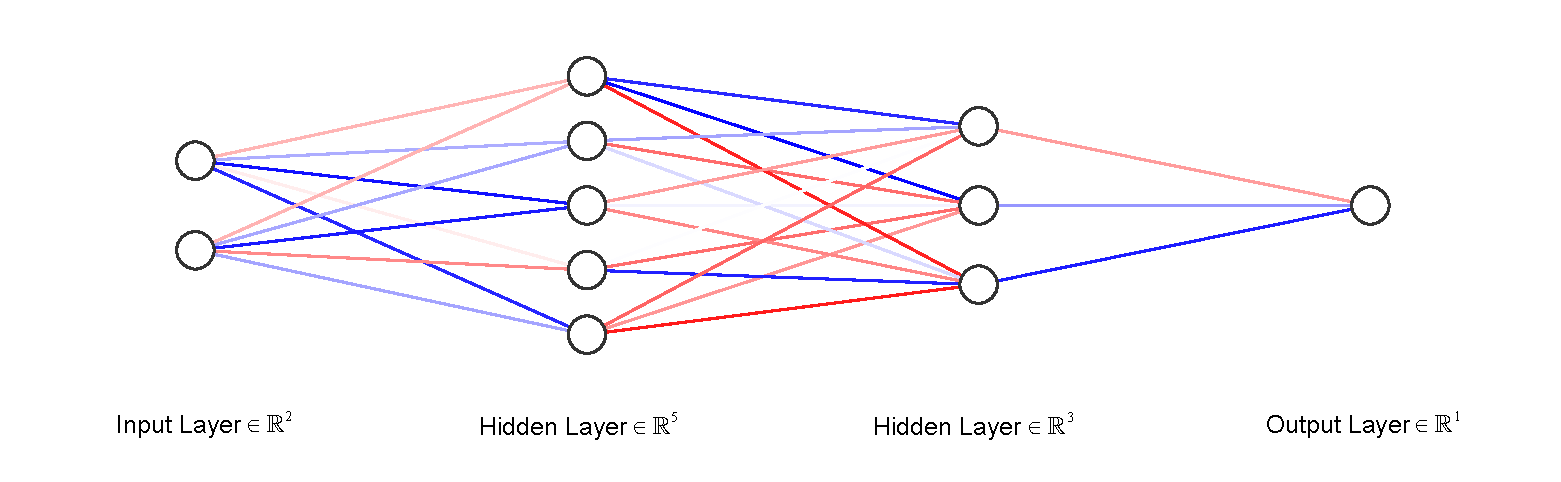
\includegraphics[width=0.99\textwidth, fbox]{Chapter2/simplenn.pdf}
\caption{Simple Neural Network}
\label{fig:simplenn} 
\end{figure}

\subsection{Back Propagation and Feedforward Network}
\label{subsec:back_propagation}

Back propagation and feedforward is based on the chain rule of derivatives. Below shows the basic chain rule. Given \autoref{eq:chainrule1} and \autoref{eq:chainrule2},

\begin{align}
    \Delta z=\frac{\partial z}{\partial y}\Delta y \label{eq:chainrule1}\\
    \Delta y=\frac{\partial y}{\partial x}\Delta x \label{eq:chainrule2}
\end{align}

The \autoref{eq:chainrule3} can be get.

\begin{equation}
\label{eq:chainrule3}
    \frac{\partial z}{\partial x}=\frac{\partial z}{\partial y} \cdot \frac{\partial y}{\partial x}
\end{equation}

One most common and basic feed forward and back propagation is shown in~\autoref{fig:backpropagation}. It has four layers, the input layer $i$, the hidden layer $j,k$ and the output layer $l$. We use this diagram to explain the feed forward and back propagation process.

When feed forward, the input data pass through the activation functions shown in~\autoref{eq:neuralunit} and calculate the output $y_l$. In the back propagation process, it utilizes the chain rule. The most beginning error gradient is $\frac{\partial E}{\partial y_l}=\Delta y$, and with the chain rule we can see: the error was accumulated along the training path, thus with given activation function, gradient in each level $G_t,t \in \{i,j,k\}$ can be derived as in~\autoref{eq:backprop} and in~\autoref{fig:backpropagation}.

\begin{equation}
\label{eq:backprop}
    G_t = \frac{\partial E}{\partial z_i},\frac{\partial E}{\partial y_k},\frac{\partial E}{\partial z_k},\frac{\partial E}{\partial y_j},\frac{\partial E}{\partial z_j}
\end{equation}

\begin{figure}[th]
\centering
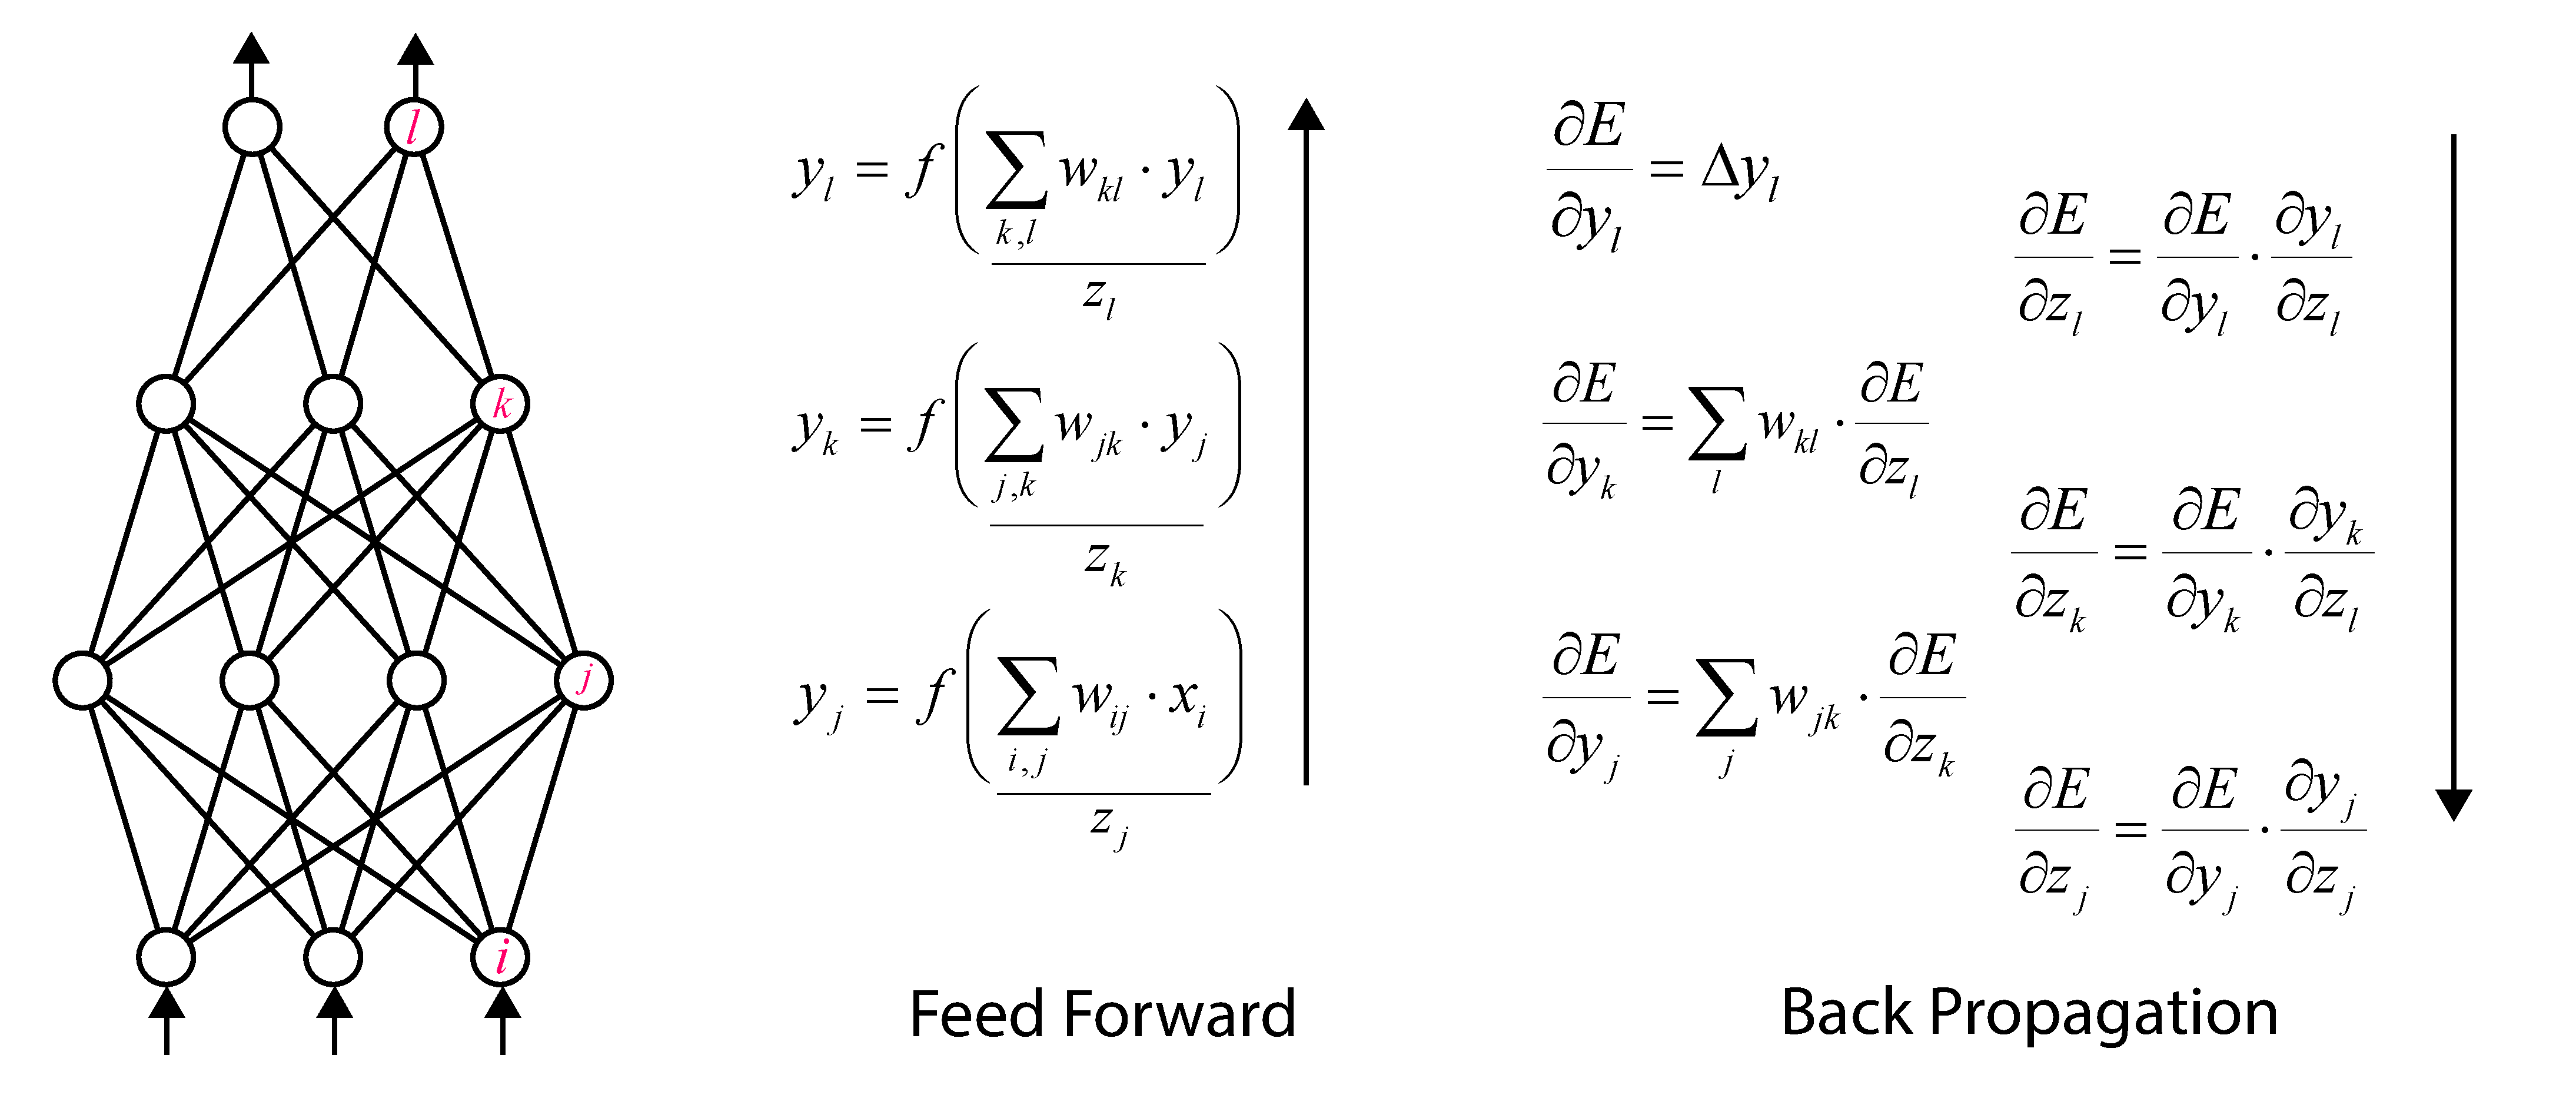
\includegraphics[width=0.99\textwidth, fbox]{Chapter2/backpropagation.pdf}
\caption{Feed Forward and Back Propagation Process}
\label{fig:backpropagation} 
\end{figure}

Notice that the each $G_t(w_{xy})$ is a linear function for weights $w_{xy}$. The aim of model is to minimize the \textit{Error} $E$. To achieve this goal, it is best to go the direction where the gradient $G_t$ decreases fastest, thus the distance $\Delta y=y_t-y_p$ between the ground-truth $y_t$ and the predicted value $y_p$ will shrink in the fastest speed.

To a conclusion, the back propagation can be described as a function $\mathbb{P}$ that

\begin{equation}
    \mathbb{P}=\argmax_{\{w\}}G_t
\end{equation}

\subsection{Application and }

Deep learning is confirmed to be solid in a variety of applications. Due to its good adaption to different domains of source data, it can fit to a any research area rapidly. Some attempt in using deep learning to address the image recognition problem go well above the previous records~\cite{krizhevsky2012imagenet, farabet2012learning, tompson2014joint, szegedy2015going}. Other areas like speech recognition~\cite{mikolov2011strategies, hinton2012deep, sainath2013deep}, natural language understanding (\textit{NLP})~\cite{collobert2011natural}, especially in recognition intelligence, like question responding~\cite{bordes2014question} and translation~\cite{jean2014using, sutskever2014sequence} also have gain surprising results. 

\begin{figure}[ht]
\centering
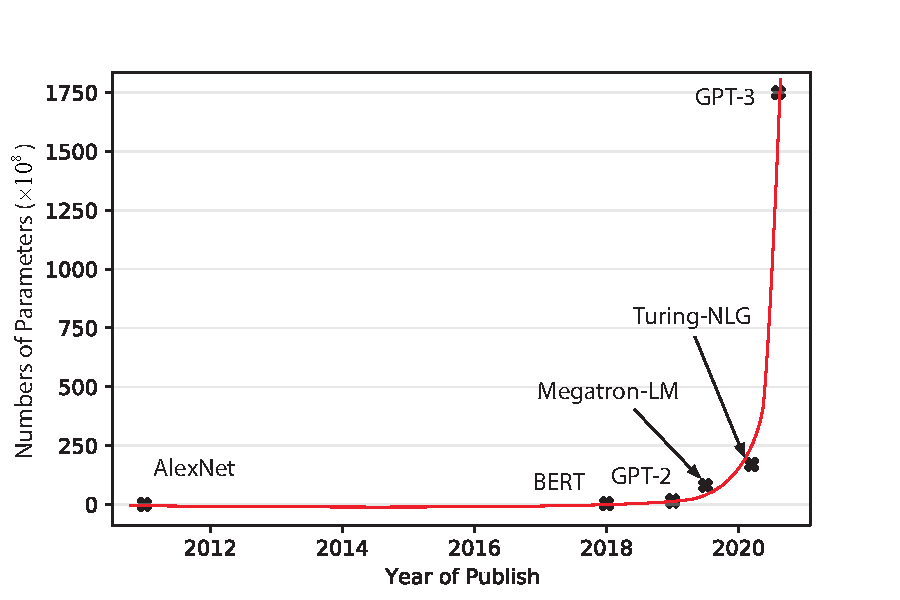
\includegraphics[width=0.99\textwidth, fbox]{Chapter2/paramnum.pdf}
\caption{Parameters of Large Scale Networks}
\label{fig:paramnum} 
\end{figure}

Besides, areas in biomedical, physics and mathematics are also using deep learning to drive their research. For example, use deep learning to find out the medical related drug components~\cite{ma2015deep}, to explore the brain circuits~\cite{helmstaedter2013connectomic} and fit the accelerator parameters~\cite{ciodaro2012online}.

The improvements of neural networks is going beyond imagination. Nowadays, researchers are not satisfied with only changing the structure of the network, but are exploring the possibility of extreme-large scale networks. ~\autoref{tab:paramnn} shows recent years development of frontier models, and their neural units used. (More neural units used, more GPU calculation resources needed.) Most recent GPT-3 consists of $1750 \times {10}^8$ parameters, which consumes OpenAI company \textit{12 Million U.S. dollars} for training. It is not realizable for any personal researcher conduct such a great amount of network. Will the future of Neural Network will fall into the 
control of few big IT companies who can afford such great cost?

\begin{table}[ht]
\caption{Parameter No. of Art-of-state Neural Networks}
\label{tab:paramnn}
\begin{tabular}{cccc}
\hline
\textbf{Network} & \textbf{Number of Parameters} & \textbf{Area}        & \textbf{Year} \\ \hline
AlexNet~\cite{krizhevsky2012imagenet}     & $0.6 \times {10}^{8}$ & Image Classification & 2011     \\
BERT~\cite{Jacob2018BERT}        & $3 \times {10}^{8}$   & Language Model       & 2018     \\
GPT-2~\cite{radford2019language}       & $15 \times {10}^{8}$  & Language Model       & 2019     \\
Megatron-LM~\cite{Shoebi2019MegatronLM} & $80 \times {10}^{8}$  & Language Model       & 2019     \\
Turing-NLG~\cite{tnlg}  & $170 \times {10}^{8}$ & Language Model       & 2020.02 \\
GPT-3~\cite{brown2020language}       & $1750 \times {10}^{8}$  & Language Model       & 2020.06 \\ \hline
\end{tabular}
\end{table}

According to DistilBERT~\cite{sanh2019distilbert}, small networks are still more flexible for more application scenarios. \autoref{fig:paramnum} shows the growth of numbers of neural parameters in recent years.

\section{Fully Convolution Networks}
\label{sec:LR_FCN}

\subsection{Convolutional Layer}

\subsection{Convolutional Neural Networks}

\section{Object Detection}
\label{sec:LR_objectdetection}



\section{Vanishing Points in Neural Networks}
\label{sec:LR_vpinNN}

\section{Concluding Remarks}

%=== END OF CHAPTER TWO ===
\end{spacing}
\newpage

%=== CHAPTER THREE (3) ===
%=== (Actual work done and contribution, including literature survey) ===

\chapter{RVPG: Refined VP Guided Lane Detection}
\label{cha:model}
\begin{spacing}{1.5}
\setlength{\parskip}{0.3in}
%  (Actual work done and contribution, including literature survey)

The next few chapters should describe the work you have done in tackling the problem. There might be a chapter on the fundamental theories relevant to the solution you are pursuing, or the supporting technologies you need in implementing the solution. Then there should be a chapter on the solution itself, followed by a chapter on the results and analysis of the results.

\section{Introduction}

say something why its strange

\section{Improved Vanishing Point Directed Neural Network}
\label{sec:MD_model}

\subsection{Overview}
The network in my work is called \textbf{RVPG Net (Refined Vanishing Point Guided Network)}. It was developed based on the VPGNet~\cite{lee2017vpgnet} and has several improvements. The network aims at detecting and classify the lanes and the road markings simultaneously, on the pixel-level. The lanes are predicted with on the guide of vanishing point. 

Multi-task combined with Convolutional Neural Network is a solid solution in traffic-sign prediction. In a research about traffic-sign design in 2016~\cite{zhu2016traffic, huval2015empirical}, researchers proposed a deep Convolutional Neural Network (CNN) structure to detect and classification those small-scaled road markings. Besides, they proposed a benchmark containing a variety of traffic signs and road markings. Because this network is good at small object detection, it can extracts the high-level features from the image, thus are more resistant to the distortion in a small area. This stability can be extended to application in rainy conditions, that the rain drop's negative effects will be offset. Based on their work, RVPG net also uses the CNN structure and multi-task method to resist the distortion of rain drop and bad illumination.

Vanishing point can direct the prediction of the curved roads. Vanishing point is the visual intersection of two parallel lines, in our case the vanishing point is the end of two converging lanes, as shown in TBC. This Vanishing Point information is utilized by human eyes, usually unconsciously, to guess the trend of the curved road. By this mechanism, human is able to predict the tendency for a long distance rather than focus only on the short distance in front of the car.

The main feature of the RVPG is the multi-task and the VP feeding. With these two design of structure, the RVPG can extract the features from the original image significantly, and it shows high accuracy \& F1-Score in the detection and classification of road markings.

\subsection{Architecture}

The architecture of the RVPG is shown in \autoref{fig:structure}. It mainly consists three stages:

\begin{enumerate} \vspace{-5mm}
    \item The convolution layers stack
    \item The multi-branch
    \item The feature combination layers stack
\end{enumerate} \vspace{-5mm}

\begin{figure}[ht]
\centering
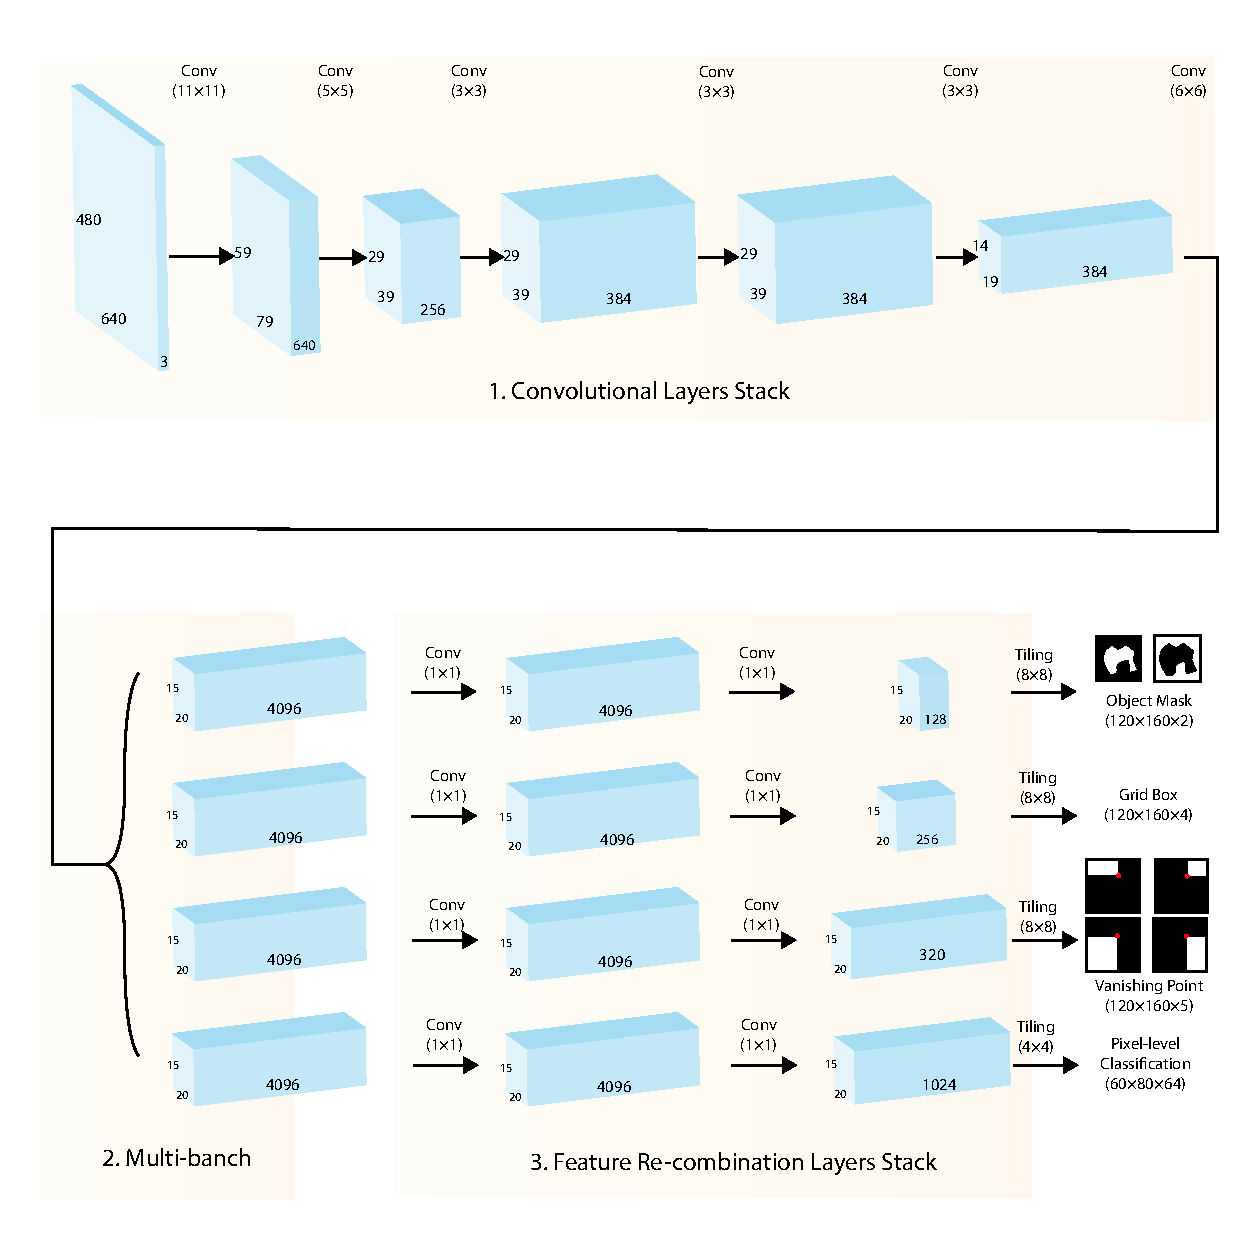
\includegraphics[width=0.99\textwidth, fbox]{Chapter3/structure.pdf}
\caption{the Structure of RVPG Network}
\label{fig:structure} 
\end{figure}

The first stage is a convolutional layer stack structure, it is aimed at extracting features. The input image is of size $480 \times 640 \times 3$\footnote{Because the relative fixde structure of network, in RVPG only 480*640 can be accepted as input. However, do re-design on network convolutional layer configuration will fit to any other size.}, in which $3$ is the RGB three color channel. Just like the CNN, the first stage of RVPG use different sizes of $2-D$ convolutional kernel to convolve the input image. In RSVP, I use the ReLU (Rectified Linear Unit, shown in \autoref{fig:relufunc}) activation function to do non-linear mapping in neutron, and the max-pooling layer to reduce the feature maps size. The target of this fist stage is to extract higher dimension of feature maps. For example, the first convolution layers' output represents the existence of the continuous edges around the object; the second convolution layers' output represents the relative position between those extracted edge features; the third convolution layers' output represents the group information of edges that are non-intersected; and so on... With deeper of the convolutional operation go, the more abstract the feature extracted are. In RVPG, five continuous convolutional layers are used in first stage.

The second stage is the multi-branch which will split the task into four different tasks simultaneously, the parameters behind the bifurcation would be shared by all tasks, but the parameters after the bifurcation would belong to each task separately. This design of multi-task have two advantages: 1) Let the different task share information. 2) Do multi-task prediction. This structure will be explained in \autoref{subsec:multitask}.

The third stage is the feature re-combination layers stack, which aims at the convergence of feature map depth towards output size. The structure in this stage is similar to CNN (As shown in lower half of \autoref{fig:structure}), but with very thick feature map layers. As can be seen, the feature map depth is $15 \times 20 \times 4096$, $15 \times 20 \times 4096$ and $15 \times 20 \times k$, in which $k \in \{128, 256, 320, 1024\}$ for different branches. Each of the convolutional layer is using $1 \times 1$ convolutional kernel. Here, the $1 \times 1$ convolutional kernel is a way to reduce out put dimension. As shown in \autoref{fig:oneonekernel}, if we want to reduce a feature map stack of size $W \times H \times N$, to $W \times H \times D, (D \neq N)$, just apply $D$ kernels of $1 \times 1 \times N$ size.

\begin{figure}[ht]
\centering
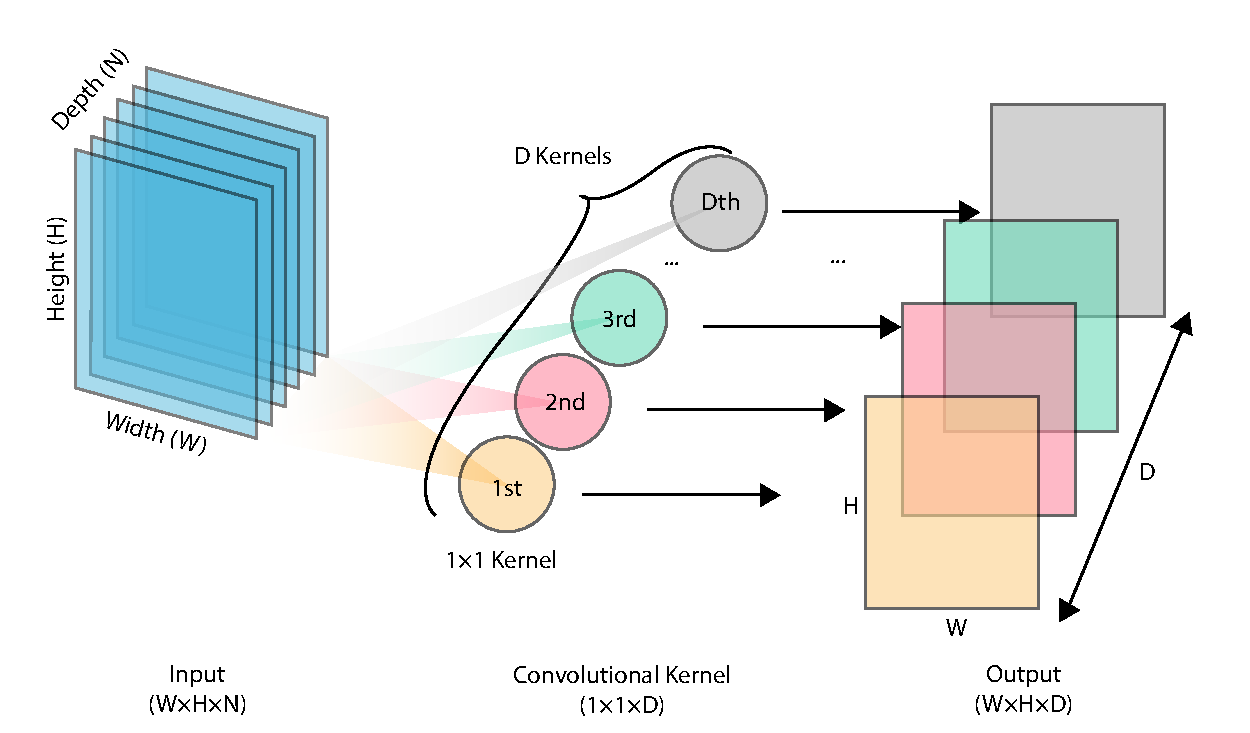
\includegraphics[width=0.99\textwidth, fbox]{Chapter3/oneonekernel.pdf} % TBC: Single kernel 1x1xN, all 1x1xNxD
\caption{Relationship between Size of Input, Kernel Num and Output}
\label{fig:oneonekernel} 
\end{figure}

The entire convolutional layers stack configuration and its index are shown in \autoref{tab:convlayer}.

\begin{table}[ht]
\centering
\caption{Convolutional Layers and Pooling Configuration}
\label{tab:convlayer}
\resizebox{\textwidth}{!}{%
\begin{tabular}{@{}ccccc@{}}
\toprule
Layer & (Kernel Size, Stride, Pad) & (Pooling Size, Stride) & Addition & Receptive Field \\ \midrule
Conv 1 & (11, 4, 0) & (3, 2) & LRN & 11 \\
Conv 2 & (5, 1, 2) & (3, 2) & LRN & 51 \\
Conv 3 & (3, 1, 1) & $-$ & $-$ & 99 \\
Conv 4 & (3, 1, 1) & $-$ & $-$ & 131 \\
Conv 5 & (3, 1, 1) & (3, 2) & $-$ & 163 \\
Conv 6 & (6, 1, 3) & $-$ & Dropout & 355 \\
Conv 7 & (1, 1, 0) & $-$ & Dropout & 355 \\
Conv 8 & (1, 1, 0) & $-$ & Branched & 355 \\ \bottomrule
\end{tabular}%
}
\end{table}

The combination of three stages can achieve four tasks at one prediction, besides, for each branch, the information learned from other branches maybe helpful to know the context of input images.

\subsection{Multi-task Structure}
\label{subsec:multitask}

Multi-task structure is the main highlight of the RVPG net. The training network are divided into four branches, each branch stands for one task in the lane and road marking, as shown in struacture diagram in \autoref{fig:structure}
% \vspace{-0mm}
\begin{align}
    F = \frac{P_{obj}}{H \times W} \times 100\% \label{eq:fore}
\end{align}
\vspace{-7mm}
\begin{equation}
    B = \frac{P_{bg}}{H \times W} \times 100\% \label{eq:bg}
\end{equation}

The first branch is the object mask task, basically a semantic detection of target object. Its output is of size $120 \times 160 \times 2$, containing 2 feature maps. In the $1$st feature map, the foreground pixels (detected objects) are set to be $1$, and other pixels are $0$. In the $2$nd feature map, the foreground pixels are set to be $0$, and the background is set to be $1$. This scheme is better than only using $1$ frame for background/foreground, because only detect the background or foreground maybe instability when either of them not easy to detect. By using both foreground and background, results can be combined for post-processing. For example, if using all-background, when the object is very small, the percentage of \autoref{eq:bg} will be very large, and the network will tend to predict all the pixels as background to achieve lower loss. In this situation, the foreground frame is very important. By using loss function like F1 score, even a small area in foreground will affect the result effectively. Thus, by combining the foreground and background 2 frames, the model will not converge at all-back or all-fore.

The second branch is the grid box branch, which is additional information for locating the objects, but finally proved to be useless. This branch is originated from VPGNet~\cite{lee2017vpgnet}. It just feeds low-definition grid boxes to the network, hopefully the network will learn to locate the object on a rough coordinate. The experimental results without this branch do not have much difference, thus we remove it in RVPG.

The third branch is Vanishing Point prediction task, in which the network will predict a $(X,Y)$ coordinate of Vanishing Point based on given image. This branch will output $120 \times 160 \times 5$ feature map. It uses $5$ channels, as 1) First channel is the VP foreground map; 2) Second channel has all pixels on the left upper corner to Vanishing point as $1$ and other pixels $0$; 3) Third channel has all pixels on the right upper corner to Vanishing point as $1$ and other pixels $0$; 4) Fourth channel has all pixels on the left lower corner to Vanishing point as $1$ and other pixels $0$; 4) Fifth channel has all pixels on the right lower corner to Vanishing point as $1$ and other pixels $0$. Details are described in \autoref{subsec:fourmap}

The fourth branch is pixel-wise classification task. For each class, the network will give a confidential value of each pixel belonging to this class. The output size is $60 \times 80 \times 64$, in which $64$ means it can predict maximum $64$ types of road markings and lanes. In the RVPG, we uses the VPG data set and Cordova data set, in which only $17$ of road markings (including lane type) types are annotated. The classes and its index are listed in \autoref{tab:classes}.

\section{Caffe Implementation}
\label{sec:MD_CAFFE}

As the original VPGNet author implements the network using CAFFE\footnote{\url{https://github.com/SeokjuLee/VPGNet}}, I also use CAFFE as my start point. But judge from the results, CAFFE is not suitable to conduct quick deep learning experiments, and I would recommend follower researchers not using CAFFE but start with PyTorch or Keras based on our code.


\subsection{Database and Extraction}

Two sets of labeled lane data are used: 1) Caltech~\cite{caltech} lanes database; 2) VPGNet~\cite{lee2017vpgnet} Lanes and road marking database. 

First and mainly used is the VPG database. In VPG database, the image are not labeled pixel-wise, but labeled with $8 \times 8$ pixels block, which complies with the output size $120 \times 160$, 

\begin{table}[ht]
\centering
\caption{Classes Specification and its Index}
\label{tab:classes}
\begin{tabular}{clcl}
\toprule
Index & Lane Type          & Index & Road Marking Type   \\ \midrule
0     & Background         & 9     & Stop Line           \\
1     & Lane Solid White   & 10    & Arrow Left          \\
2     & Lane Broken White  & 11    & Arrow Right         \\
3     & Lane Double White  & 12    & Arrow Go Straight   \\
4     & Lane Solid Yellow  & 13    & Arrow U Turn        \\
5     & Lane Broken Yellow & 14    & Speed Bump          \\
6     & Lane Double Yellow & 15    & Cross Walk          \\
7     & Lane Broken Blue   & 16    & Safety Zone         \\
8     & Lane Slow          & 17    & Other Road Markings \\ \bottomrule
\end{tabular}
\end{table}%

\subsection{Environment Configuration}

CAFFE version etc table

\subsection{Training Data Preprocessing}



\subsection{4-Map: Vanishing Point Feeding Scheme}
\label{subsec:fourmap}

Why use, how to, what achieved.

\section{PyTorch Implementation}
\label{sec:MD_PyTorch}

\subsection{Motivation}

The drawback is severe: 1) CAFFE needs C++ debugging, which takes long time to compile each time. As a large network like VPGNet, it usually takes more than $10$ mins per compilation. 2) CAFFE is not friendly in document support, and lacks the user-friendly API, thus you need to go into all the C++ underlying code before do any change, even the most basic layer definition change. 3) CAFFE's support of GPU and CUDA suite is out-of-date, thus sometimes with the newest computer with RTX 3080 GPU, you may even not able to call the GPU support with CAFFE.

In a conclusion, don't use CAFFE anymore.

\subsection{Data Format Conversion}

\subsection{4-Tilling: Redesigned Tilling Layer}



\section{Improvements}
\label{sec:MD_improvement}
\setlength{\parskip}{0.3in}

\subsection{2-D Gaussian}
\label{subsec:IM_2D}

\subsection{Res Blocks}
\label{subsec:IM_resblock}

\subsection{E-Net}
\label{subsec:IM_Enet}



\section{Concluding Remarks}




%=== END OF CHAPTER THREE ===
\end{spacing}
\newpage

%=== CHAPTER FOUR (4) ===
%=== Test and Experiments ===

\chapter{Test and Experiments}
\begin{spacing}{1.5}
\setlength{\parskip}{0.3in}

\section{One}

\section{Two}

\section{Three}


%=== END OF CHAPTER FOUR ===
\end{spacing}
\newpage

%=== CHAPTER FIVE (5) ===
%=== Discussion ===

\chapter{Experimental Results and Discussion}
\label{cha:experiments}
\begin{spacing}{1.5}
\setlength{\parskip}{0.3in}

\section{Introduction}

\section{Test Metrics}

\section{Multi-class Visualization Tool}

\section{Multi-class Performance}

\section{Rainy Condition}

\section{Post-processing}

\subsection{Selection of Confidential Threshold}

\subsection{Contour}

\section{Concluding Remarks}

%=== END OF CHAPTER FIVE ===
\end{spacing}
\newpage

%=== CHAPTER SIX (6) ===
%=== Conclusion and Recommendations ===

\chapter{Conclusion and Recommendations}
\label{cha:conclusion}
\begin{spacing}{1.5}
\setlength{\parskip}{0.3in}

\section{Conclusions}

Highlight the significance of the results, and perhaps the consequences of the results, critically where necessary.

\section{Recommendation in Future Work}

\subsection{Detection under Rainy Condition}

Identify the inadequacies of what you have done, and suggest how the gaps may be plugged.

\subsection{Improvements on Few Sample Road Markings}


%=== END OF CHAPTER SIX ===
\end{spacing}
\newpage

%==== ENDING PART ===

\bibliographystyle{unsrt}
\begin{spacing}{1.5}
\bibliography{Ref/References}
\end{spacing}
\newpage

%=== APPENDIX ===
%=== APPENDIX ===
\chapter*{Appendix A}
\label{cha:appendixa}
\fancypagestyle{addin}{
\fancyhead[R]{\bf \textsl{APPENDIX A} \vspace{0.1in}}
}
\thispagestyle{addin}
\addcontentsline{toc}{chapter}{Appendix A}
\setlength{\parskip}{0.3in}
% \begin{spacing}{1.5}


% \end{spacing}
\clearpage

\chapter*{Appendix B}
\fancypagestyle{addin}{
\fancyhead[R]{\bf \textsl{APPENDIX B} \vspace{0.1in}}
}
\pagestyle{addin}
\addcontentsline{toc}{chapter}{Appendix B}
\begin{spacing}{1.5}

(Code Here)

Usually codes lah.

\end{spacing}
%=== END OF CHAPTER SIX ===
\newpage
%==== END OF ALL ===
\end{document}
